% Options for packages loaded elsewhere
\PassOptionsToPackage{unicode}{hyperref}
\PassOptionsToPackage{hyphens}{url}
\PassOptionsToPackage{dvipsnames,svgnames*,x11names*}{xcolor}
%
\documentclass[
  11pt,
]{article}
\usepackage{lmodern}
\usepackage{setspace}
\usepackage{amsmath}
\usepackage{ifxetex,ifluatex}
\ifnum 0\ifxetex 1\fi\ifluatex 1\fi=0 % if pdftex
  \usepackage[T1]{fontenc}
  \usepackage[utf8]{inputenc}
  \usepackage{textcomp} % provide euro and other symbols
  \usepackage{amssymb}
\else % if luatex or xetex
  \usepackage{unicode-math}
  \defaultfontfeatures{Scale=MatchLowercase}
  \defaultfontfeatures[\rmfamily]{Ligatures=TeX,Scale=1}
\fi
% Use upquote if available, for straight quotes in verbatim environments
\IfFileExists{upquote.sty}{\usepackage{upquote}}{}
\IfFileExists{microtype.sty}{% use microtype if available
  \usepackage[]{microtype}
  \UseMicrotypeSet[protrusion]{basicmath} % disable protrusion for tt fonts
}{}
\makeatletter
\@ifundefined{KOMAClassName}{% if non-KOMA class
  \IfFileExists{parskip.sty}{%
    \usepackage{parskip}
  }{% else
    \setlength{\parindent}{0pt}
    \setlength{\parskip}{6pt plus 2pt minus 1pt}}
}{% if KOMA class
  \KOMAoptions{parskip=half}}
\makeatother
\usepackage{xcolor}
\IfFileExists{xurl.sty}{\usepackage{xurl}}{} % add URL line breaks if available
\IfFileExists{bookmark.sty}{\usepackage{bookmark}}{\usepackage{hyperref}}
\hypersetup{
  pdftitle={Semiparametric estimation for time series: a frequency domain approach based on optimal transportation theory},
  colorlinks=true,
  linkcolor=Maroon,
  filecolor=Maroon,
  citecolor=Blue,
  urlcolor=blue,
  pdfcreator={LaTeX via pandoc}}
\urlstyle{same} % disable monospaced font for URLs
\usepackage[margin=1in]{geometry}
\usepackage{graphicx}
\makeatletter
\def\maxwidth{\ifdim\Gin@nat@width>\linewidth\linewidth\else\Gin@nat@width\fi}
\def\maxheight{\ifdim\Gin@nat@height>\textheight\textheight\else\Gin@nat@height\fi}
\makeatother
% Scale images if necessary, so that they will not overflow the page
% margins by default, and it is still possible to overwrite the defaults
% using explicit options in \includegraphics[width, height, ...]{}
\setkeys{Gin}{width=\maxwidth,height=\maxheight,keepaspectratio}
% Set default figure placement to htbp
\makeatletter
\def\fps@figure{htbp}
\makeatother
\setlength{\emergencystretch}{3em} % prevent overfull lines
\providecommand{\tightlist}{%
  \setlength{\itemsep}{0pt}\setlength{\parskip}{0pt}}
\setcounter{secnumdepth}{5}
\usepackage{caption}
\captionsetup[figure]{font=footnotesize,margin=9pt,labelfont=bf,textfont=it}
\captionsetup[table]{font=footnotesize,margin=9pt,labelfont=bf,textfont=it}
\ifluatex
  \usepackage{selnolig}  % disable illegal ligatures
\fi
\newlength{\cslhangindent}
\setlength{\cslhangindent}{1.5em}
\newlength{\csllabelwidth}
\setlength{\csllabelwidth}{3em}
\newenvironment{CSLReferences}[2] % #1 hanging-ident, #2 entry spacing
 {% don't indent paragraphs
  \setlength{\parindent}{0pt}
  % turn on hanging indent if param 1 is 1
  \ifodd #1 \everypar{\setlength{\hangindent}{\cslhangindent}}\ignorespaces\fi
  % set entry spacing
  \ifnum #2 > 0
  \setlength{\parskip}{#2\baselineskip}
  \fi
 }%
 {}
\usepackage{calc}
\newcommand{\CSLBlock}[1]{#1\hfill\break}
\newcommand{\CSLLeftMargin}[1]{\parbox[t]{\csllabelwidth}{#1}}
\newcommand{\CSLRightInline}[1]{\parbox[t]{\linewidth - \csllabelwidth}{#1}\break}
\newcommand{\CSLIndent}[1]{\hspace{\cslhangindent}#1}

\title{Semiparametric estimation for time series: a frequency domain
approach based on optimal transportation theory}
\author{Manon Felix\\
Advisor: Prof.~Davide La Vecchia}
\date{May 2021}

\begin{document}
\maketitle
\begin{abstract}
In this master thesis, we make use of some results available in the
optimal transportation literature to develop a novel methodology for
parameters estimation in time series models. The key idea is to use the
Wasserstein distance and Sinkhorn divergence to derive minimum distance
(or divergence) estimators for short- and long-memory time series
models. Working on the (discrete) Fourier transform of a time series we
conduct inference in the frequency domain: we compute the
distance/divergence between the empirical distribution of the
standardized periodogram ordinates and their theoretical distribution,
as implied by standard asymptotic theory. To study the properties of
these new estimators, we perform several Monte-Carlo simulations. Our
numerical results suggest that the estimators belonging to our novel
class are root- \(n\) consistent. Their performance, in terms of Mean
Squared-Error, is similar to the one yielded by the state-of-the-art
estimation method (Whittle's estimator) in the case of short- and
long-memory Gaussian process. For short-memory processes and long-memory
processes, in the presence of outliers our estimators outperform the
Whittle's estimator as well as when the underlying innovation density of
a long-memory process is skewed.
\end{abstract}

\setstretch{1.5}
\newpage

\tableofcontents

\newpage

\hypertarget{introduction}{%
\section{Introduction}\label{introduction}}

\hypertarget{motivation}{%
\subsection{Motivation}\label{motivation}}

The aim of this master thesis is to combine some results from optimal
transport theory with the statistical analysis time series analysis.
Working with the frequency domain approach, we aim at developing a novel
methodology for estimating the parameters of a univariate stochastic
process.

We do not rely on the standard information divergence-based methods,
among which the standard maximum likelihood estimator approach, and
consider instead the mathematical theory of optimal measure
transportation.

The optimal transport theory has been applied in many research areas,
like e.g.~mathematics, differential geometry, partial differential
equations and applied mathematics (see e.g.
\protect\hyperlink{ref-santambrogio2015optimal}{Santambrogio}
(\protect\hyperlink{ref-santambrogio2015optimal}{2015}) and
\protect\hyperlink{ref-villani2009optimal}{Villani}
(\protect\hyperlink{ref-villani2009optimal}{2009})). The Wasserstein
distance is also useful for contrasting complex objects and can be
applied to signal processes and engineering (see e.g.
\protect\hyperlink{ref-kolouri2017optimal}{Kolouri et al.}
(\protect\hyperlink{ref-kolouri2017optimal}{2017})). Many data analysis
techniques in computer vision, imaging (e.g.~for color/texture
processing or histograms comparisons), and more general machine learning
problems about regression, classification, and generative modeling are
often based on optimal transportation theory (see
\protect\hyperlink{ref-peyre2019computational}{Peyré, Cuturi, and
others} (\protect\hyperlink{ref-peyre2019computational}{2019})). For an
overview on statistical use of the optimal transportation see
\protect\hyperlink{ref-panaretos2020invitation}{Panaretos and Zemel}
(\protect\hyperlink{ref-panaretos2020invitation}{2020}) and for a
book-length discussion see
\protect\hyperlink{ref-ambrosio2013user}{Ambrosio and Gigli}
(\protect\hyperlink{ref-ambrosio2013user}{2013}). Recently, the
Wasserstein distance has become popular specially for inference in
generative adversarial networks (see e.g.,
\protect\hyperlink{ref-arjovsky2017wasserstein}{Arjovsky, Chintala, and
Bottou} (\protect\hyperlink{ref-arjovsky2017wasserstein}{2017})).

However, to the best of our knowledge, only a limited number of papers
has been investigating the use of the optimal transport theory in the
statistical analysis of time series analysis (see
\protect\hyperlink{ref-ni2020conditional}{Ni et al.}
(\protect\hyperlink{ref-ni2020conditional}{2020})); we refer to
\protect\hyperlink{ref-bernton2019parameter}{Bernton et al.}
(\protect\hyperlink{ref-bernton2019parameter}{2019}) for a survey of the
Wasserstein distance for statistical inference. Our purpose is to fill
this gap in the literature and study the applicability of the
Wasserstein distance (or, more generally, of some results from optimal
transportation theory) for the statistical analysis of time series, via
frequency domain techniques. The key argument for moving from the time
domain to the frequency domain is that we are dealing with data that are
independent and identically distributed (i.i.d). The assumption of
i.i.d. data facilitates, as it is often the case in statistics, the
estimation of parameters in a model.

We propose a novel class of minimum distance estimator (see e.g.
\protect\hyperlink{ref-basu2019statistical}{Basu, Shioya, and Park}
(\protect\hyperlink{ref-basu2019statistical}{2019}) for a book-length
introduction) by minimizing the distance between the theoretical and
empirical distribution of the standardized periodogram ordinates (SPOs).
This program is supported by the fact that the method to replace the
maximum likelihood estimator with minimum Wasserstein distance has
already been applied, for instance in astronomy and climate science (see
\protect\hyperlink{ref-bernton2019parameter}{Bernton et al.}
(\protect\hyperlink{ref-bernton2019parameter}{2019})). Additionally,
consistency properties of estimators based on the Wasserstein distance
has already been studied by
\protect\hyperlink{ref-bassetti2006minimum}{Bassetti, Bodini, and
Regazzini} (\protect\hyperlink{ref-bassetti2006minimum}{2006}) and
\protect\hyperlink{ref-bernton2019parameter}{Bernton et al.}
(\protect\hyperlink{ref-bernton2019parameter}{2019}). In our case, we
study the properties (bias, variance, consistency, etc.) of our new
estimators by means of Monte-Carlo experiments and compare them to the
state-of-the-art estimator, the Whittle's estimator (see
\protect\hyperlink{ref-whittle1953estimation}{Whittle}
(\protect\hyperlink{ref-whittle1953estimation}{1953})). We analyze our
results for several types of distribution (standard, heavy-tailed and
skewed) and focusing on both large and small samples. We believe that
our results are promising and open the possibility of further research.

\hypertarget{organization}{%
\subsection{Organization}\label{organization}}

The thesis has the following structure. In the first chapter, we review
the main concepts of the optimal transport theory and provide the
definitions and key mathematical tools necessary to understand our
methodological development. In the second chapter, we briefly recall the
Whittle's estimation theory and the key related results. Then, we
introduce our novel estimators and compare them to the Whittle's
estimator. We conclude mentioning some possible research's directions
which can make use of this thesis as a stepston. The R-codes needed to
reproduce the exercises/plots/tables included in this thesis are
available on Github at the link
\url{https://github.com/ManonFelix/Semidiscrete_estimation_ts}.

\hypertarget{measure-transportation}{%
\section{Measure transportation}\label{measure-transportation}}

This chapter aims to explain the main principles behind the theory of
optimal transport. The original formulation of the optimal transport
problem was given by \protect\hyperlink{ref-monge1781memoire}{Monge}
(\protect\hyperlink{ref-monge1781memoire}{1781}). He proposed a way to
calculate the most effective strategy for moving a large amount of sand
from one place to another with the least amount of effort required. In
mathematical terms, given a source measure \(\mu\), target measure
\(\nu\) supported on sets \(X\) and \(Y\) respectively and a
transportation cost function \(c(x,y)\) the goal is to find a transport
map \(T:X \rightarrow Y\) such as

\[\min _{\nu=T_{\#} \mu} \int_{X} c(x, T(x)) \mathrm{d} \nu(x)\]

where the constraint
\(\mu(T^{-1}(A)) = \nu(A) \implies \nu=T_{\#} \mu \ , \forall A\)
ensures that all the mass from \(\mu\) is transported to \(\nu\) by the
map \(T\).

The notation \(\nu=T_{\#} \mu\) means that the map \(T\) pushes forward
\(\mu\) to a new measure \(\nu\) and therefore \(T_{\#}\) is called the
pushforward operator.

Monges problem (defined using \(c(x, y)=|x-y|)\) remained open until the
\(1940 \mathrm{~s}\), when it was revisited by
\protect\hyperlink{ref-kantorovich1942translocation}{Kantorovich}
(\protect\hyperlink{ref-kantorovich1942translocation}{1942}). In his
reformulation, he seeks for a transport plan and allows mass splitting.
Therefore, he proposed to compute how much mass gets moved from \(x\) to
\(y\) and define a joint measure (a coupling)
\(\pi \in \mathcal{P}\left(\mathbb{R}^{d}, \mathbb{R}^{d}\right)\) which
satisfies for all \(A, B \in \mathcal{B}\left(\mathbb{R}^{d}\right)\):
\(\pi\left(A \times \mathbb{R}^{d}\right)=\mu(A), \ \pi\left(\mathbb{R}^{d} \times B\right)=\nu(B).\)
We denote by \(\Pi(\mu, \nu)\) the set of transport plans between
\(\mu\) and \(\nu\) (i.e.~couplings). Then, \(p\)-Wasserstein distance
is defined as

\begin{equation}
W_{p}(\mu, \nu)=\left(\min _{\pi \in \Pi(\mu, \nu)} \int_{\mathbb{R}^{d} \times \mathbb{R}^{d}}|x-y|^{p} d \pi(x, y)\right)^{\frac{1}{p}}.
\label{eq:wass_p}
\end{equation}

Obtaining a closed-form expression for \(W_{p}\) is typically
impossible. However, the case of one dimensional probability densities,
say \(f_{S}(x)\) and \(f_{T}(x)\) with cumulative distribution functions
\(F_{S}(x)\) and \(F_{T}(x)\), is specifically interesting as the
\(p = 1\) Wasserstein distance (a.k.a the Earth Mover's Distance,
henceforth EMD) has the following expression

\begin{equation}
\mathcal{W}_{1}(\mu, \nu)=\int_{\mathbb{R}}\left|F_{S}(x)-F_{T}(x)\right| d x
\label{eq:wass_1}
\end{equation}

The possibility of using this closed-formed solution to conduct
inference on time series motivates the thesis.

Beyond the EMD, other measure transportation related diverges can be
explored to conducted inference. In this thesis we consider the version
of the Wasserstein distance:

\begin{equation}
W_{\lambda}(\mu, \nu) =\int_{x, y} c(x, y) \mathrm{d} \pi(x, y)+ \lambda \int \log \left(\frac{\pi(x, y)}{\mathrm{d} \mu(x) \mathrm{d} \nu(y)}\right) \mathrm{d} \pi(x, y). 
\label{eq:sink}
\end{equation}

as introduced by \protect\hyperlink{ref-cuturi2013sinkhorn}{Cuturi}
(\protect\hyperlink{ref-cuturi2013sinkhorn}{2013}). Minimizing Eq.
\ref{eq:sink} leads to the so called Sinkhorn divergence. This
divergence is obtained adding to the original optimal transportation
problem an entropic regularization term (right part). When \(\lambda\)
is small, the Sinkhorn divergence approximates the Wasserstein distance.
However, in contrast to the Wasserstein distance, the regularized
Sinkhorn divergence is differentiable and smooth, so it yields some
computational advantages in terms of optimization problems.

\hypertarget{inference-in-the-frequency-domain}{%
\section{Inference in the frequency
domain}\label{inference-in-the-frequency-domain}}

Before introducing our estimators, let us first provide an overview of
the theory that is commonly applied to conduct inference on time series
models in the frequency domain.

Consider a stationary process \(\{Y_t\}\) of \(n\) observations
\(y_{1:n} = y_1, … ,y_n\). We focus on linear time series \(\{Y_t\}\)
satisfying

\[
\phi(L)(1-L)^{d} Y_{t}=\varphi(L) \epsilon_{t}
\]

where \(LX_t = X_{t-1}\) (back shift operator). \(\phi(z)\) and
\(\varphi(z)\) are the auto-regressive and moving average polynomial of
order \(p\) and \(q\) respectively. The time series \(\{Y_t\}\) may or
may not have long memory depending on the value of \(d\). When
\(0 < d < 0.5\) the process is called a long-memory process and are
extensively applied in finance (see e.g
\protect\hyperlink{ref-tsay2005analysis}{Tsay}
(\protect\hyperlink{ref-tsay2005analysis}{2005})) . In the literature,
we often rewrite \(d\) as \(H = d +1/2\), which is called Hurst
exponent.

Our setting is of \emph{semiparametric nature}: we have an Euclidean
parameter \(\theta\) characterizing the auto-regressive and moving
average polynomials and the long memory, but we do not assume any
distribution for the innovation term \(\epsilon_{t}\) (so the innovation
density is an infinite dimensional nuisance parameter). For the sake on
numerical illustration, we present our results for the case when
\(\epsilon_{t} \sim N\left(0, \sigma_{\epsilon}^{2}=1\right)\) but also
underlying innovation densities with fatter tails (like e.g.~Skew t (see
\protect\hyperlink{ref-azzalini2003distributions}{Azzalini and
Capitanio} (\protect\hyperlink{ref-azzalini2003distributions}{2003}))
and Student t).

To conduct inference on the model parameters
\(\theta=\left(\sigma_{\epsilon}^{2}, d, \phi_{1}, \ldots, \phi_{p}, \varphi_{1}, \ldots, \varphi_{q}\right)\)
of long-memory processes, we could assume that \(\epsilon_t\) is
normally distributed and rely on pseudo (or quasi) MLE. Thanks to this
assumption, we can write the likelihood of the process and optimize it
to find \(\hat \theta\), which under suitable assumptions remains
root-\(n\) consistent and asymptotically normal; see e.g.
\protect\hyperlink{ref-gourieroux1995statistics}{Gourieroux and Monfort}
(\protect\hyperlink{ref-gourieroux1995statistics}{1995}). Nevertheless,
this approach is extremely time-consuming and can even be unfeasible due
to the strong dependence and long-memory properties of the process. A
solution to this inference issue relies on tackling the problem in the
frequency domain and work on the discrete Fourier transform of
\(\{Y_t\}\). This is the frequency domain proposed by Whittle and the
key idea is to represent a time series as combination of cos/sinusoids.

The main tool utilized in the frequency domain is the spectral density.
The spectral density \(f(\lambda_j, \theta)\) of \(Y_t\)

\[
f(\lambda_j, \theta)=\left|1-e^{i \lambda}\right|^{-2 d}\frac{\sigma_{\epsilon}^{2}}{2 \pi} \frac{|\varphi(\exp \{-i \omega\})|^{2}}{|\phi(\exp \{-i \omega\})|^{2}}
\] where \(\varphi(x)=1-\sum_{k=1}^{p} \varphi_{k} x^{k}\) and
\(\phi(x)=1+\sum_{k=1}^{q} \phi_{k} x^{k}\). \(\lambda_j\) are the
fundamental Fourier frequencies where
\(\lambda_j=2 \pi(j / n), j \in \mathcal{J}=\{1,2, \ldots,[(n-1) / 2]\}\).

The spectrum of a time series can be estimated by the method of moment.
Its sample analogue is called the periodogram

\[I\left(\lambda_{j}\right)=\frac{1}{2 \pi n}\left|\sum_{t=1}^{n}\left(Y_{t}-\bar{Y}_{n}\right) e^{i t \lambda_{j}}\right|^{2}.\]

The periodogram is asymptotically unbiased. Nevertheless, it is an
inconsistent estimator; see e.g.
\protect\hyperlink{ref-priestley1981spectral}{Priestley}
(\protect\hyperlink{ref-priestley1981spectral}{1981}). Moreover, a key
result showed by
\protect\hyperlink{ref-priestley1981spectral}{Priestley}
(\protect\hyperlink{ref-priestley1981spectral}{1981}) and
\protect\hyperlink{ref-brillinger2001time}{Brillinger}
(\protect\hyperlink{ref-brillinger2001time}{2001}) is that the
periodogram ordinates are asymptotically independent and exponentially
distributed with rate equal to the spectral density. In other words, the
standardized periodogram ordinates (henceforth, SPOs) are asymptotically
independent and have an exponential distribution with rate one:

\[\frac{I(\lambda_j)}{f(\lambda_j, \theta)}  \stackrel{d}{\rightarrow} i . i . d . Exp(1).\]

This idea was introduced and exploited by Whittle
(\protect\hyperlink{ref-whittle1953estimation}{Whittle}
(\protect\hyperlink{ref-whittle1953estimation}{1953})), who proposed to
minimize the Whittle approximated likelihood:

\begin{equation}
L_{W}(\theta)=\frac{1}{2 \pi}\left[\int_{-\pi}^{\pi} \ln f(\lambda, \theta) d \lambda+\int_{-\pi}^{\pi} \frac{I(\lambda)}{f(\lambda, \theta)} d \lambda\right]
\label{eq:Whittle}
\end{equation}

which is derived from the fact that the SPOs are asymptotically
identically distributed according to an exponential distribution.

To implement the Whittle's estimator, Eq. \ref{eq:Whittle} can be
rewritten by separating the variance component from the rest of the
parameters vector as

\begin{equation}
L_{W}\left(\theta^{*}\right)=\sum_{j \in \mathcal{J}} \frac{I\left(\lambda_{j}\right)}{f\left(\lambda_{j}, \theta^{*}\right)}
\end{equation}

where
\(f\left(\lambda_{j}, \theta^{*}\right)=2 \pi \sigma_{\epsilon}^{2} f\left(\lambda_{j}, \theta^{*}\right)\)
and
\(\theta^{*}=\left(1, \eta=\left(d, \phi_{1}, \ldots, \phi_{p}, \varphi_{1}, \ldots, \varphi_{q}\right)\right)\).
The following minimization problem (which hinges on the notion of
concentrated likelihood) can be set up to find Whittle estimator; see
e.g. \protect\hyperlink{ref-beran1994statistics}{Beran}
(\protect\hyperlink{ref-beran1994statistics}{1994}) for a book-length
discussion. First, minimize

\[\arg \min _{\eta} L_{W}\left(\theta^{*}\right)=\arg \min _{\eta} L_{W}(\eta)\]

which yields to \(\hat{\eta}\). Then, set

\[\hat{\sigma}_{\epsilon}^{2}=2 \pi L_{W}(\hat{\eta}).\]

One can prove (see e.g.
\protect\hyperlink{ref-beran1994statistics}{Beran}
(\protect\hyperlink{ref-beran1994statistics}{1994})) the consistency of
the parameter \(\hat \theta^*\). Additionally, the parameter is
root-\(n\) consistent and converges to a normal distribution. In the
case of underlying Gaussian innovation terms, \(\hat \theta\) achieves
the Cramer-Rao lower bound. The Whittle's estimator is routinely applied
to long- and short-memory time series, like e.g.~ARMA(\(p,q\)) proces,
and it is still consistent and asymptotically normal. We therefore use
this estimation method as our reference to compare our results with the
state-of-the-art methodology.

\hypertarget{methodology}{%
\section{Methodology}\label{methodology}}

\hypertarget{problem-settings}{%
\subsection{Problem settings}\label{problem-settings}}

Our goal is to find the parameter \(\eta = \theta^*\) of a time series
model in the parameter space \(\theta^* \in \Theta\) with dimension
\(\Theta \subset \mathbb{R}^{s}\), with \(s \geq 1\), that minimizes the
distance between the empirical and theoretical cumulative distributions
of the SPOs. We denote the distance or divergence used by
\(\mathcal{D}\) and write our minimum distance estimator such as

\[\hat{\theta^*}=\underset{\theta^* \in \Theta}{\text{arg min}} \ \mathcal{D}\left({\mu}, \nu_{\theta^*}\right) .\]

where \(\mu\) is the theoretical exponential distribution and
\(\nu_{\theta^*}\) is the empirical distribution of the SPOs. We denote
the SPOs of a time series \(X_1, ..., X_m\) where
\(X \sim \nu_{\theta^*}\). In our study, several estimators are
considered and each of them yields an estimator.

In our exposition, we redefine \(\mathcal{D}\) in each optimization
problem. For instance, when \(\mathcal{D}\) is the Wasserstein distance,
we denote the corresponding minimum Wasserstein estimator (MWE) as
\(\hat \theta^*_{MWE}\). For the sake of simplicity, we assumed the
variance of the innovation term \(\sigma^2_\epsilon\) to be known and
equal to one. Hence, our parameter vector to be estimated is
\(\theta^* = (d, \phi_{1}, \ldots, \phi_{p}, \varphi_{1}, \ldots, \varphi_{q}).\)
In addition to that, we focus first on processes with underlying
Gaussian distribution and then extend to other distributions with fat
tails and/or contaminated by outliers.

\hypertarget{estimation-methods}{%
\subsection{Estimation methods}\label{estimation-methods}}

\hypertarget{minimum-wasserstein-estimator}{%
\subsubsection{Minimum Wasserstein
Estimator}\label{minimum-wasserstein-estimator}}

The Wasserstein distance when \(p=1\) is given in Eq. \ref{eq:wass_1}
when \(F_{\nu} = F_{\theta^*}\) is the empirical cumulative distribution
of the SPOs, we estimate it by \[
\hat{F}_{\theta^*}(x)=\frac{1}{m} \sum_{j=1}^{m} \mathbf{1}_{X_{j} \leq x}
\] where
\(X_j(\theta^*) = I(\lambda_j) / f\left(\lambda_{j}, \theta^*\right)\)
for \(j = 1, ..., m\) are the SPOs of a time series process
asymptotically independent and exponentially distributed.

To compute \(F_\mu\), as it is common in machine learning literature
about generative models, we initially thought to generate exponential
random variables and stack then in a vector (\(Z\), say). In
mathematical terms, for a sample size \(n\), we generate
\([(n-1)/2] = m\) observations \(z_1, ..., z_m\) of random variables
\(Z_1, ..., Z_m\) following an exponential distribution with rate one
and store them in a vector \(Z\). Since \(p = 1\) in Eq. \ref{eq:wass_p}
and we work on univariate time series, the Wasserstein distance can be
approximated by

\begin{equation}
\mathcal{D}(\mu, \nu_{\theta^*}) = \frac{1}{m} \sum_{j = 1}^{m} |x_j - z_j| 
\label{eq:wass_1_app}
\end{equation}

where \(x_j\) are the SPOs asymptotically exponentially distributed
depending on the parameter vector \(\theta^*\) through the spectral
density function \(f(\lambda_j, \theta^*)\) and \(z_j\) are the
observations generated using \(Z \sim Exp(1)\). Minimizing Eq.
\ref{eq:wass_1_app} leads to the minimum Wasserstein estimator noted \[
\hat \theta^*_{MWE} = \underset{\theta^*}{\text{arg min}} \  \mathcal{D}(\mu, \nu_{\theta^*}).
\] Figure \ref{fig:wasserstein_farima} displays the Wasserstein loss
function of two FARIMA(\(0,d,0\)) processes. The top plot shows a smooth
and concave loss function with a global minimum that is the same value
as the Whittle's estimator's. On the other hand, the bottom plot shows a
wiggly function around the true value of the parameter.

\begin{figure}

{\centering 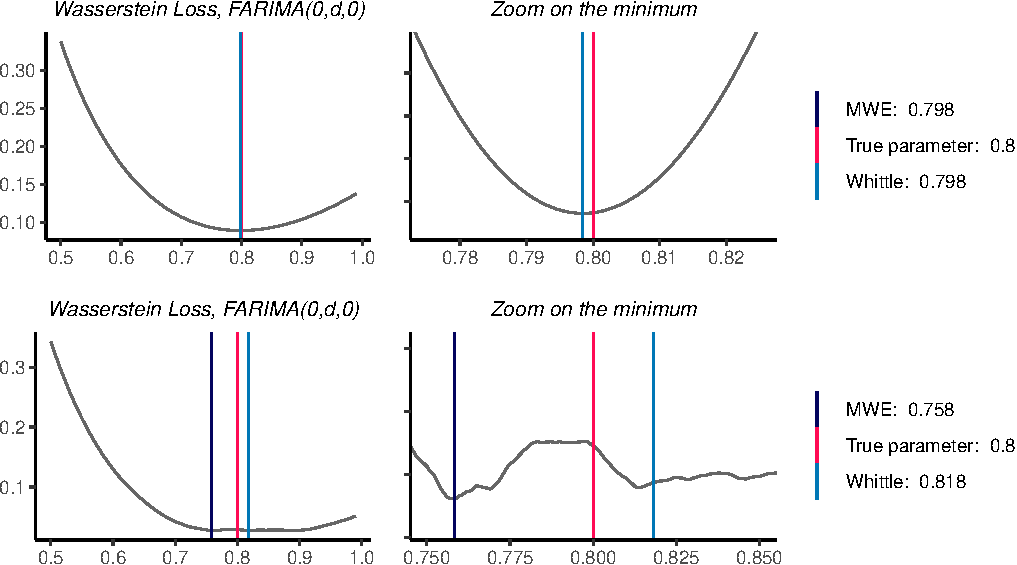
\includegraphics[width=0.6\linewidth]{Master_thesis_V4_files/figure-latex/wasserstein_farima-1} 

}

\caption{Wasserstein loss functions of two FARIMA(0,d,0) processes where H = 0.8 (d = 1.2). The sample size is 3001. The left column display the entire loss functions for all possible parameter values that a long-memory process can take (0.51 < H < 0.99). The right column is a zoom on the functions.}\label{fig:wasserstein_farima}
\end{figure}

Thus, if one uses the Wasserstein loss to estimate the parameter \(d\),
these two phenomena arise: we end up with either a smooth function
containing a global minimum or a function that fluctuates and has
several local minima.

Through this thesis, we tackle these issues and introduce estimators
that are defined by loss functions which do not suffer from these
problems.

Our first finding is that the computed distance might vary widely around
the true parameter value and its value depends heavily on the sample
simulated from an Exp(1), i.e.~\(z_1, ..., z_m\). As a consequence, the
estimated model parameter(s) \(\hat \theta_{MWE}\) typically depends
heavily on the random exponential variables generated to conduct the
optimization.

To illustrate the problem, on Figure \ref{fig:wasserstein_z} we continue
with the process used to plot the bottom plots of Figure
\ref{fig:wasserstein_farima} and simply change the seed with which the
vector \(Z\) is generated. We remark that we are now dealing with a loss
function that is smooth and has a global minimum that is precisely the
true value of the parameter \(\theta^* = H = 0.8\). Therefore, we see
that by modifying the vector \(Z\), we can obtain a more appropriate
loss function. We find this aspect potentially problematic for numerical
optimization: by definition a random vector cannot be controlled and we
may obtain biased estimates simply because of the simulated variables
needed for the optimization procedure.

\begin{figure}[h]

{\centering 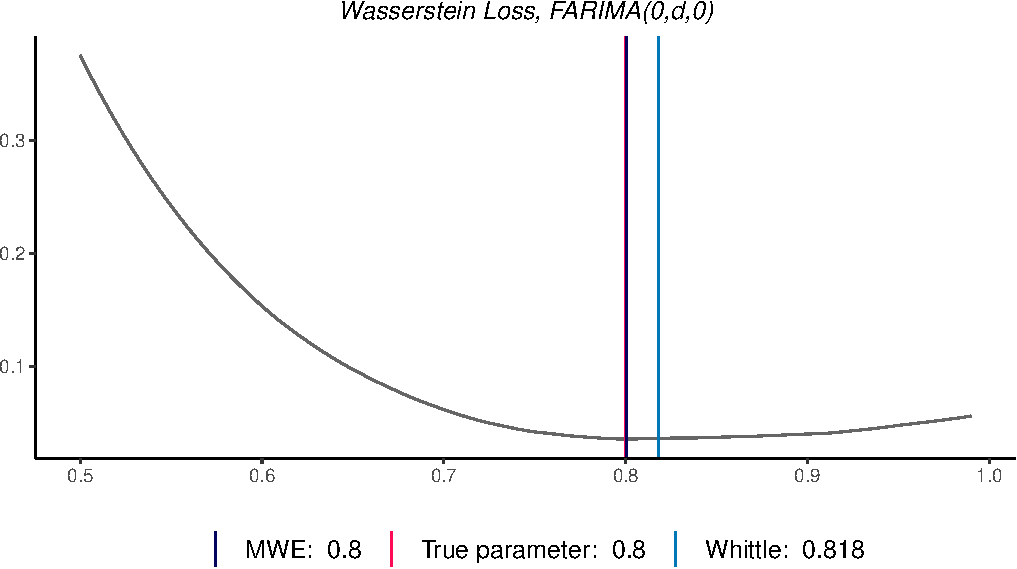
\includegraphics[width=0.55\linewidth]{Master_thesis_V4_files/figure-latex/wasserstein_z-1} 

}

\caption{Wasserstein loss function of the FARIMA(0,d,0) process (bottom one) of Figure 1 computed with another random vector.}\label{fig:wasserstein_z}
\end{figure}

In order to get a better overview of the behavior of the minimum
Wasserstein estimator when the vector \(Z\) changes, we compute
\(k = 200\) times \(\hat \theta^*_{MWE}\) for a given process of size
\(n = 3001\). Then, we plot the results on Figure \ref{fig:MWE_n}. We
can observe that, even for large sample size, the estimated parameter
depends heavily on the random vector \(Z\). Nevertheless, the mean
remains relatively close to the true value.

\begin{figure}[h]

{\centering 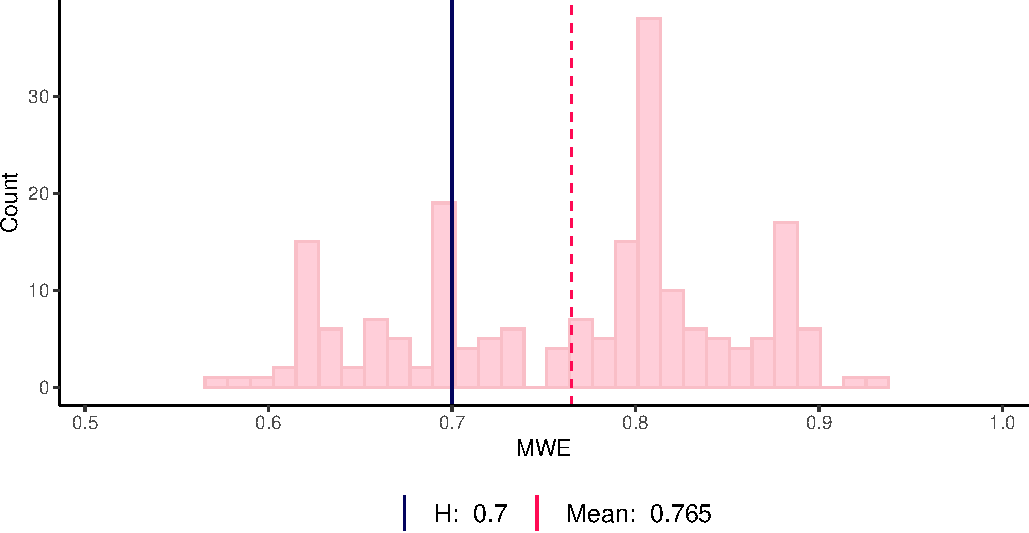
\includegraphics[width=0.6\linewidth]{Master_thesis_V4_files/figure-latex/MWE_n-1} 

}

\caption{We simulate 200 vectors following an exponential distribution and then compute the MWE of a FARIMA(0,d,0) process with n = 3001. The blue line is the true parameter H = 0.7 value and the red dashed line is the mean of the MWE.}\label{fig:MWE_n}
\end{figure}

To cope with this problem of dependence between the random vector \(Z\)
and the parameter estimate, we are going to explore two options.

\hypertarget{option-a-mean-of-minimum-wasserstein-estimators}{%
\subsubsection{Option A: Mean of Minimum Wasserstein
Estimators}\label{option-a-mean-of-minimum-wasserstein-estimators}}

For each simulated times series, we generate several exponential random
variables and stack them in vectors. Then, we estimate the model
parameter for each of the simulated vector and report the mean of the
estimated parameter.

For illustration, based on the same process than in Figure
\ref{fig:MWE_n} with \(n = 3001\), we generate
\(k = 10, 20 , 50, 100 , 200, 500, 1000\) random vectors, estimate the
\(k\) parameters and then report the mean. Thus, the mean becomes our
estimator and we note it \(\hat \theta^*_{MMWE}\). The results are
listed in Table \ref{tab:MWE_k}. As \(k\) increases, the average becomes
progressively closer to the true parameter.

\begin{table}[h]
\centering
\begin{tabular}{|c|c|c|c|c|c|c|c|c|}
\hline
$k$ &  1 & 10   & 20    & 50    & 100   & 200   & 500   & 1000 \\
\hline
$\hat \theta^*_{MMWE}$ & 0.807 & 0.73 & 0.727 & 0.726 & 0.721 & 0.719 & 0.714 & 0.714 \\
\hline
\end{tabular}
\caption{Mean of the minimum Wasserstein estimators for a FARIMA($0,d,0$) of size $n = 3001$ by varying the value of $k$, i.e. the number of exponential random vectors generated. The true value is 0.7.}
\label{tab:MWE_k}
\end{table}

\hypertarget{option-b-minimum-semidiscrete-wasserstein-estimator}{%
\subsubsection{Option B: Minimum Semidiscrete Wasserstein
Estimator}\label{option-b-minimum-semidiscrete-wasserstein-estimator}}

Instead of using the empirical cumulative distribution function (c.d.f)
of exponential random variables generated from a computer, we plan to
use the c.d.f of exponential variables with rate one for the SPOs,
namely \(F(x)=1-e^{-x}\). Therefore, the Wasserstein distance becomes:

\begin{equation}
\int_\mathcal{X}\left|\hat F_{\theta^*}(x)- (1 - e^{-x})\right| \mathrm{d} x 
\end{equation}

where
\(\hat F_{\theta^*}(x) = \frac{1}{m} \sum_{j=1}^{m} \mathbf{1}_{X_{j} \leq x}\)
and \(X_j (\theta^*)\) are the SPOs of a process. To compute this distance, we
replace
\(\hat F_\mu(z) = \frac{1}{m}\sum_{j=1}^{m} \mathbf{1}_{Z_{j} \leq z}\)
by \(F_\mu = 1 - e^{-x}\). We use a trapezoidal integration to
approximate the integral and name the estimator minimum semidiscrete
Wasserstein estimatior (MSWE), i.e.~\(\hat \theta^*_{MSWE}\). Thanks to
this second option, there is no longer randomness in our process
estimation. The corresponding loss functions for two FARIMA(\(0,d,0\))
processes using this method are showed in Figure \ref{fig:semi_wass}

\begin{figure}

{\centering 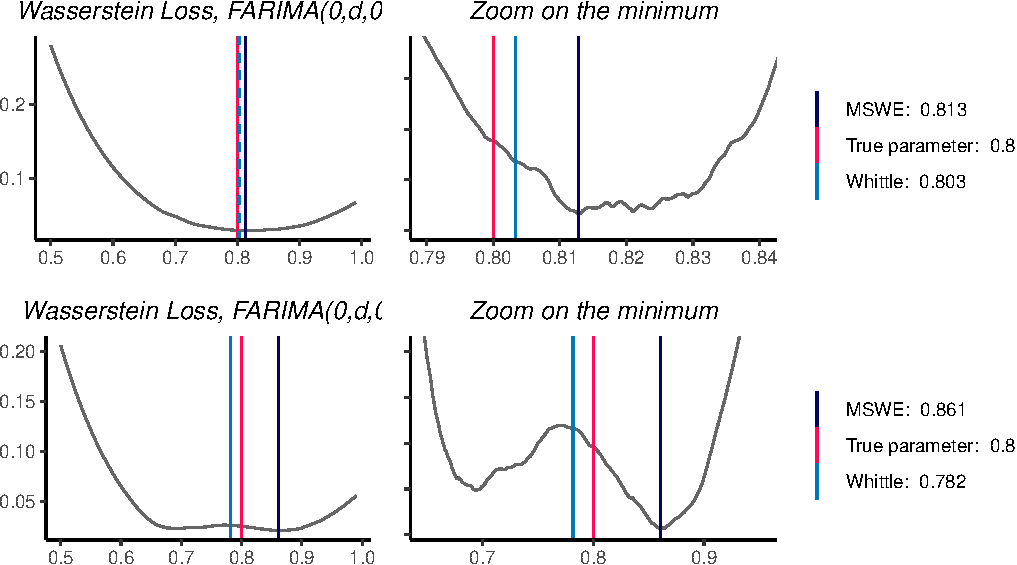
\includegraphics[width=0.6\linewidth]{Master_thesis_V4_files/figure-latex/semi_wass-1} 

}

\caption{Semidiscrete Wasserstein loss functions for two FARIMA(0,d,0) processes. The sample size is 3001 and the true parameter value is 0.8.}\label{fig:semi_wass}
\end{figure}

Still, another problem persists. The Wasserstein loss, even for large
sample size, is often not well-shaped (i.e smooth and concave): it may
contain several local minima (see e.g.~Figure
\ref{fig:wasserstein_farima} and Figure \ref{fig:semi_wass}). This fact
entails biased estimates with large variance. It should also be noted
that the loss shape degenerates even more when \(n\) decreases (see
Figure \ref{fig:small_sample}). So far, we are not able to explain why
there is such diversity in the shape of the loss functions and we are
planning to investigate theoretically this point.

\begin{figure}

{\centering 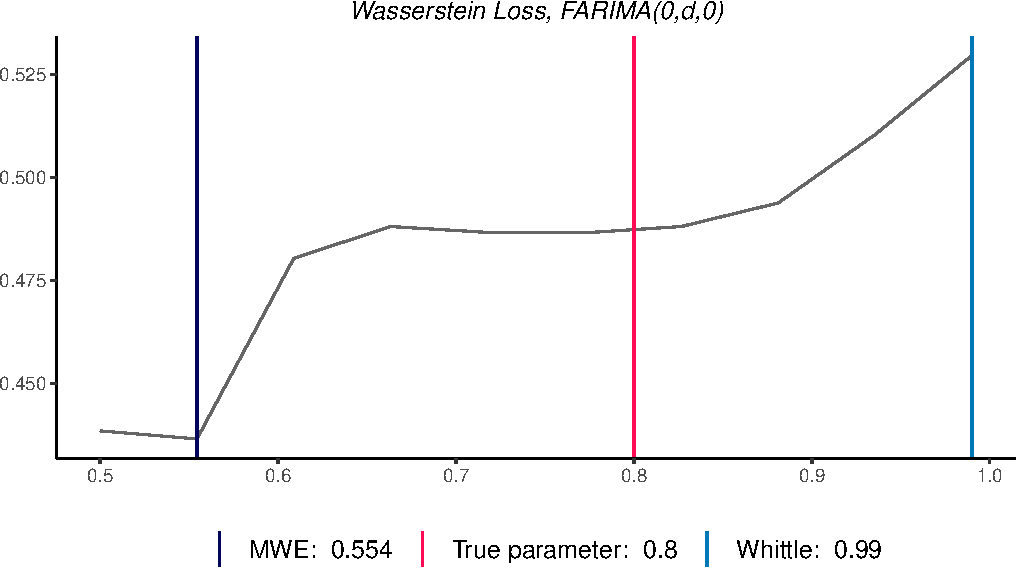
\includegraphics[width=0.5\linewidth]{Master_thesis_V4_files/figure-latex/small_sample-1} 

}

\caption{Wasserstein loss function of a FARIMA(0,d,0) process with sample size equal to 51.}\label{fig:small_sample}
\end{figure}

\hypertarget{minimum-weighted-wasserstein-estimator}{%
\subsubsection{Minimum Weighted Wasserstein
Estimator}\label{minimum-weighted-wasserstein-estimator}}

In our numerical experiments, we realized that by inserting some weights
in the loss function defined by the Wasserstein distance yields a much
more regular function to optimize. Therefore, we introduce another class
of minimum divergence estimators which are related to the minimization
problem of Eq. \ref{eq:wass_1} where the empirical cumulative
distribution of the SPOs \(\hat F_\nu(x) = \hat F_{\theta^*}(x)\) is
given by

\[\hat F_{\theta^*}(x)=\sum_{j=1}^{m} w_{j} 1\left\{X_{j} \leq x\right\}\]

where
\(X_{j}\left(\theta^{*}\right)=I\left(\lambda_{j}\right) / f\left(\lambda_{j}, \theta^{*}\right)\)
for \(j=1, \ldots, m\) are the SPOs of a time series process and the
associated weights \(\{w_j\}\) are

\begin{equation}
w_j = \frac{\frac{I(\lambda_j)}{f(\lambda_j; \theta)}}{\sum^m_{j = 1}\frac{I(\lambda_j)}{f(\lambda_j; \theta)}}.
\label{eq:weights}
\end{equation}

We call the estimator solution to the minimization problem in Eq.
\ref{eq:weights} the minimum weighted Wasserstein estimator; we will use
the acronym MWWE and the notation \(\theta^*_{MWWE}\).

To implement the MWWE we resort on some optimization routines already
available in the statistical software (R). Most of these routines
require that the weights sum up to \(1\) and that are comprised between
\(0\) and \(1\). Therefore, we propose the use of the weights in Eq.
\ref{eq:weights}.

In order to give an intuition for the employment of these weights, we
report in Figure \ref{fig:qqplot} a Quantile-Quantile plot. These are
the quantiles of the SPOs of a FARIMA(\(0,d = 0.8,0\)) processcomputed
by substituting \(\theta = \hat \theta^*_{Whittle} = 0.818\) and
\(\theta = \hat \theta^*_{MWE} = 0.742\) against the quantiles of an
exponential distribution with rate one. We notice that the SPOs from the
minimum Wasserstein distance estimation method have an heavy tailed
distribution than those from Whittle's estimation method (see
\ref{fig:qqplot}. This phenomenon is not an isolated case and often the
Wasserstein's SPOs have this feature. Intuitively, the weights proposed
give more leverage to extreme values while computing the Wasserstein
distance and therefore prevents the SPOs selected by the Wasserstein
distance minimization method from being too extreme in value and too far
from an exponential distribution with rate one.

\begin{figure}

{\centering 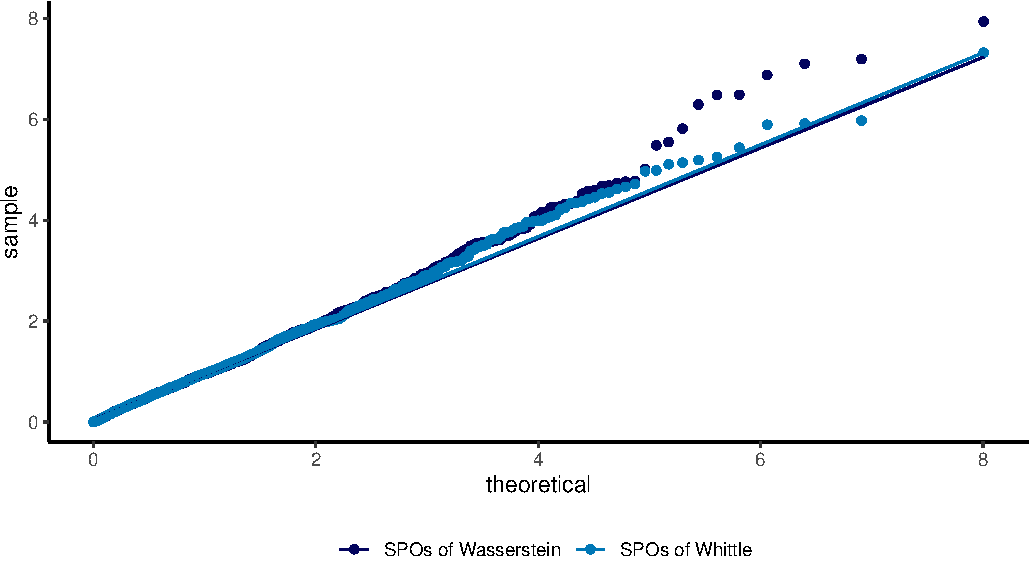
\includegraphics[width=0.6\linewidth]{Master_thesis_V4_files/figure-latex/qqplot-1} 

}

\caption{Qqplot of the Wasserstein's SPOs and the Whittle's SPOs. The SPOs are from a long-memory process with H = 0.8 and the sample size is equal to 3001.}\label{fig:qqplot}
\end{figure}

Figure \ref{fig:weighted_wasserstein} shows the plot of the loss
function for same process and vector \(Z\) as Figure
\ref{fig:wasserstein_farima}, but now we apply the weights to calculate
our weighted Wasserstein distance. We see that the weighted Wasserstein
loss function is smooth and contains a minimum which is even closer to
the true parameter than the one obtained optimizing the Whittle's loss
function.

\begin{figure}

{\centering 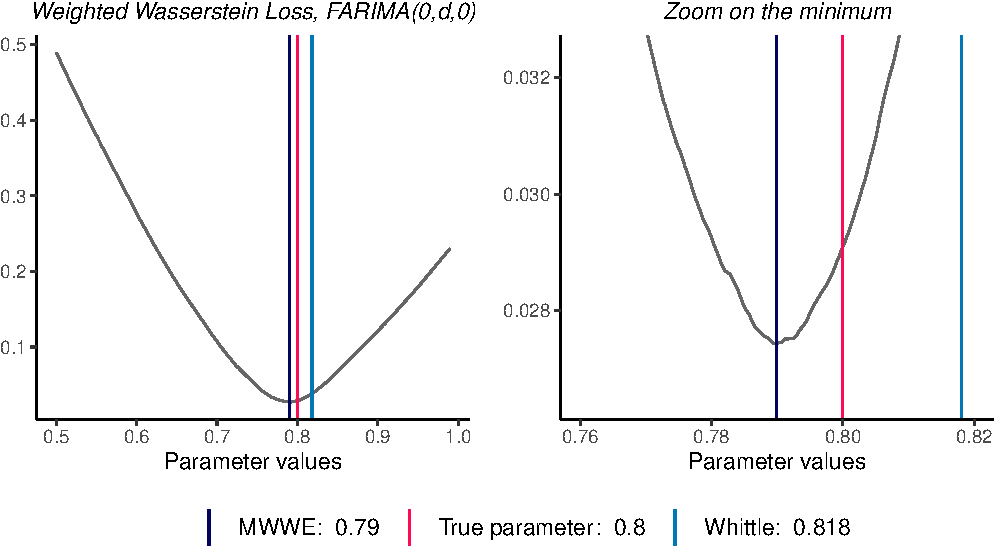
\includegraphics[width=0.6\linewidth]{Master_thesis_V4_files/figure-latex/weighted_wasserstein-1} 

}

\caption{Weighted Wasserstein loss function of the FARIMA(0,d,0) process on Figure 1 (bottom).}\label{fig:weighted_wasserstein}
\end{figure}

We remark that the weights applied here are not optimal: the problem of
selecting optimal (in some asymptotic sense, like e.g.~minimum trace of
the asymptotic variance) weights remains open and it will be the object
of our future research. Nevertheless, the weights proposed in this
section work well especially for ARMA(\(p,q\)) processes as illustrated
on Figure \ref{fig:wass_ar1_weighted}. The shape of the loss function
using the weighted Wasserstein estimator suggests that we could obtain
an estimator with small variance---this is intuition is gained looking
at the convexity of the loss function in a neighbourhood of the true
parameter value. Moreover, we are also thinking of implementing the
minimum expected Wasserstein estimator defined by
\protect\hyperlink{ref-bernton2019parameter}{Bernton et al.}
(\protect\hyperlink{ref-bernton2019parameter}{2019}). Also this research
topic will be investigated in future research.

\begin{figure}

{\centering 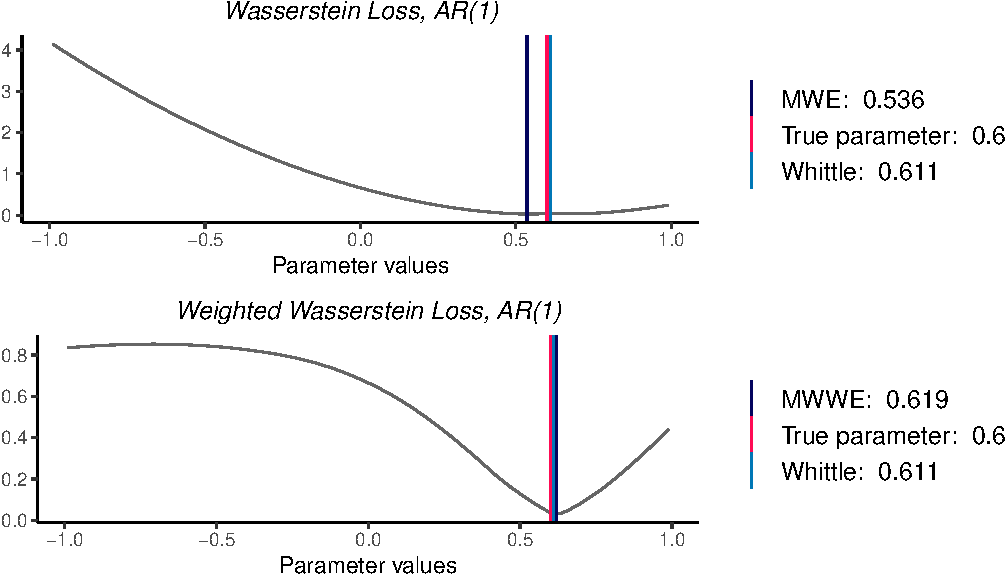
\includegraphics[width=0.6\linewidth]{Master_thesis_V4_files/figure-latex/wass_ar1_weighted-1} 

}

\caption{Wasserstein loss function and weighted Wasserstein loss function of a Gaussian AR(1) process. The sample size is 3001 and the true parameter is 0.6.}\label{fig:wass_ar1_weighted}
\end{figure}

\hypertarget{minimum-sinkhorn-estimator}{%
\subsubsection{Minimum Sinkhorn
Estimator}\label{minimum-sinkhorn-estimator}}

A second idea is to employ the Sinkhorn divergence (see Eq.
\ref{eq:sink}) to estimate our parameter based on
\protect\hyperlink{ref-cuturi2013sinkhorn}{Cuturi}
(\protect\hyperlink{ref-cuturi2013sinkhorn}{2013}). We conjecture that
the regularization term should have an impact on the shape of the loss
function, making it smoother. To check numerically this conjecture, in
Figure \ref{fig:sinkhorn}, we compare the loss function of the
Wasserstein distance with the one related to the Sinkhorn divergence. We
see that we deal with a smooth and concave function, whose minimum is
very close to the true value. The picture illustrates another good
property of the Sinkhorn divergence is that it remains smooth even for a
very small sample size.

\begin{figure}

{\centering 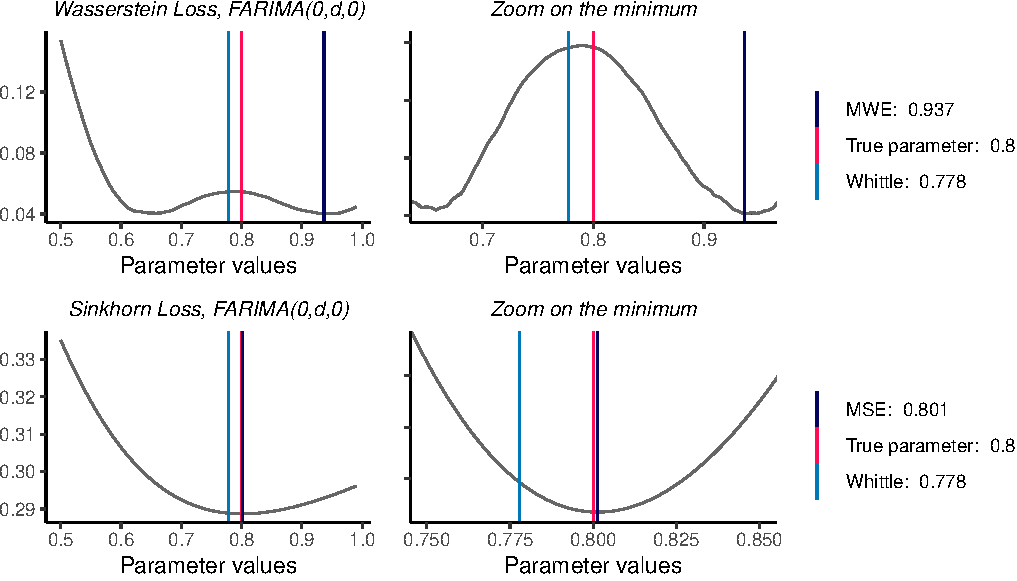
\includegraphics[width=0.65\linewidth]{Master_thesis_V4_files/figure-latex/sinkhorn-1} 

}

\caption{Top: Wasserstein loss function of a FARIMA(0,d,0) process. Bottom: Sinkhorn loss function of the same process. The sample size is 1801.}\label{fig:sinkhorn}
\end{figure}

Nevertheless, the use of the Sinkhorn divergence raises an important
question: which value(s) to select for \(\lambda\)? In order to choose
the optimal (in a sense that we are going to clarify) \(\lambda\), we
suggest to implement classical machine learning techniques to perform
model selection, such as the cross validation (leave-one-out); see for
example \protect\hyperlink{ref-friedman2001elements}{Friedman et al.}
(\protect\hyperlink{ref-friedman2001elements}{2001}) Chapter 7.

To illustrate, we randomly divide a time series into \(2\) groups
\(C_1 \ (80\%), C_2 \ (20\%)\) also called folds. We treat the first
group as train and the second group as validation/test. For a selection
of \(\lambda\), we estimate our parameter, the minimum Sinkhorn
estimator (MSKE), on the train set and then use the corresponding
\(\hat \theta_{MSKE}\) to predict the time data of our test set.

For the sake-of-exposition, we illustrate the procedure using an AR(1)
process, \(Y_t = \phi_1 Y_{t-1} + \epsilon_t\) where
\(\epsilon_t \sim N(0,1)\) and \(\theta^* = \phi_1 = 0.6\). After
estimating the parameter thanks to the train set, we substitute its
value in \(\hat \epsilon_t = Y_t - \hat \theta^*_{MSKE} Y_{t-1}\) where
\(t = 2, ..., l\). \(l\) is the length of the testing vector and depends
on which ratios we choose to split our time process \({Y_t}\) in our
case \(80\% - 20\%\). Then, we compute the empirical prediction error
\(err_\lambda\) for a given \(\lambda\):

\[err_{\lambda} \textit{ of the test set} = \frac{1}{l}\sum_{t = 2}^l \hat \epsilon_t^2 = \frac{1}{l} \sum_{t = 2}^l (Y_t - \hat \theta^*_{MSKE} Y_{t-1})^2\]

We repeat this method for several lambda values and plot the results on
Figure \ref{fig:SH_CV}. The minimum testing error is achieved when
\(\lambda = 0.1\), to which corresponds
\(\hat \theta^*_{MSKE_{\lambda = 0.1}} = 0.572\)- a value close to the
true parameter value \(\theta^* = 0.6\).

\begin{figure}

{\centering 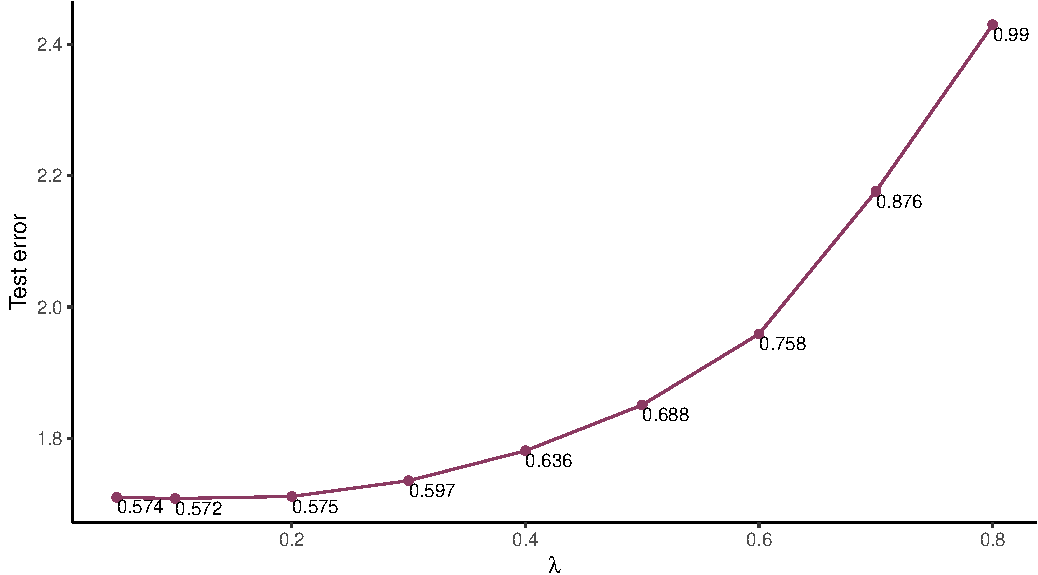
\includegraphics[width=0.55\linewidth]{Master_thesis_V4_files/figure-latex/SH_CV-1} 

}

\caption{Testing MSE vs lambda values for an AR(1) process. The sample size is 4001 and the true parameter value is 0.6. For this process, the minimum emprical prediction error is achieved when lambda = 0.1.}\label{fig:SH_CV}
\end{figure}

\hypertarget{results}{%
\section{Results}\label{results}}

\hypertarget{monte-carlo-simulations}{%
\subsection{Monte Carlo Simulations}\label{monte-carlo-simulations}}

In this section we run a horse race among the different estimators
presented in the previous sections. Our criterion for evaluating the
performance of each of the estimators is the Mean Squared Error
(\(MSE\))

\[MSE(\hat \theta^*, \theta^*) = \mathbb{E}(\theta^*-\hat{\theta^*})^{2} = \operatorname{Var}(\hat{\theta^*})+\operatorname{Bias}^{2}(\hat \theta^*, \theta^*)\]

where
\(Bias(\hat \theta^*, \theta^*) = \mathrm{E}[\hat \theta^*] - \theta^*\)
and
\(Var( \hat \theta^*) = \mathrm{E}[(\hat \theta^*)^2]-\mathrm{E}[\hat \theta^*]^{2}\).
The MSE represents the bias-variance trade-off which typically emerges
in statistics when it comes to model selection. To obtain approximations
of the MSE, bias and variance of \(\hat \theta^*\) we compute

\[\widehat{MSE}(\hat \theta^*, \theta^*) =  \frac{1}{B}\sum_{b = 1}^{B}(\hat \theta^*_b - \theta^*)^2,\]
\[\widehat{Bias}(\hat \theta^*, \theta^*) = \hat \theta^{* \cdot} - \theta^*,\]
\[\widehat{Var}( \hat \theta^*) \frac{1}{B - 1} \sum^{B}_{b = 1}(\hat \theta^*_b - \hat \theta^{* \cdot})^2\]

where \(B\) is the number of Monte Carlo simulations, i.e.~the number of
simulated processes, and
\(\hat \theta^{* \cdot} = \frac{1}{B} \sum^B_{b = 1} \hat \theta^*_b\).

\hypertarget{long-memory-process}{%
\subsubsection{Long-memory Process}\label{long-memory-process}}

Firstly, we simulate \(B = 400\) stationary FARIMA(\(0,d,0\)) processes
of size \(n = 3201\) and \(H = 0.8 \ (d = 0.3)\) according to

\[(1-L)^{0.3}Y_t = \epsilon_t.\]

For each process, we compute the Whittle's estimator
\(\hat \theta^*_{WH}\), the minimum Wasserstein estimator
\(\hat \theta^*_{MWE}\), the mean of the minimum Wasserstein estimators
\(\hat \theta^*_{MMWE, \ k}\), the minimum semidiscrete Wasserstein
estimator \(\hat \theta^*_{MSWE}\), the minimum weighted Wasserstein
estimator \(\hat \theta^*_{MWWE}\) and the minimum Sinkhorn estimator
\(\hat \theta^*_{MSKE,\ \lambda}\). Figure \ref{fig:box_farima_400}
reports the results.

\begin{figure}

{\centering \includegraphics[width=0.6\linewidth]{/Users/manonfelix/OneDrive/Master thesis/Redaction/images/box_400_farima_gauss} 

}

\caption{Boxplots of all the estimators presented during this thesis. The sample size of the 400 simulated Gaussian FARIMA(0,d,0) is 3201 and d = 0.3 (H = 0.8).}\label{fig:box_farima_400}
\end{figure}

We note that the minimum Wasserstein estimator has very high variance
due to the problems mentioned earlier. By using the mean of the minimum
Wasserstein estimators we can reduce the variance and the bias of the
minimum Wasserstein estimator (see Table \ref{tab:farima_mse_gaussian})
while using the minimum semidiscrete Wasserstein estimator allows to
reduce the bias. Our minimum weighted Wasserstein estimator is similar
to Whittle's estimator in terms of Mean Squared Error: both estimators
have small variance and a bias close to \(0\) (see Table
\ref{tab:farima_mse_gaussian}). We zoom on the density of these two
estimators and we display it in Figure \ref{fig:density_long_gauss}. We
see that both distributions are centered around the true parameter and
have similar shape. Nevertheless, the minimum weighted Wasserstein
estimator has larger tails, which entails a larger variance.

The use of the Sinkhorn distance seems promising but depends on the
\(\lambda\) parameter. When \(\lambda\) is equal to \(0.1\), the minimum
Sinkhorn estimator is well centered around the true parameter and has a
reasonable variance. Here, we do not choose \(\lambda\) by
cross-validation because of the time needed for computation. We compute
the Sinkhorn distance where the value of \(\lambda\) is determined in
advance. It is expected that by performing a selection of lambda
parameters we will obtain even better results.

\begin{figure}

{\centering \includegraphics[width=0.6\linewidth]{/Users/manonfelix/OneDrive/Master thesis/Redaction/images/density_long} 

}

\caption{Distribution of the Whittle's estimator and the weighted Wasserstein estimator estimated with the 400 simulations of Figure 11.}\label{fig:density_long_gauss}
\end{figure}

\begin{table}[h]
\centering
\begin{tabular}{|l|c|c|c|}
\hline
\textbf{Distribution}                   & \multicolumn{3}{c|}{\textbf{Gaussian}}                                                            \\ \hline
\textbf{}                               & $\widehat{MSE}( \hat \theta^*)$ & $\widehat{Bias}( \hat \theta^*)$ & $\widehat{Var}( \hat \theta^*)$ \\ \hline
$\hat \theta^*_{Whittle}$               & 0.00018                        & -0.00164                         & 0.00018                        \\ \hline
$\hat \theta^*_{MWE}$                   & 0.00425                        & -0.01207                         & 0.00411                        \\ \hline
$\hat \theta^*_{MMWE, \ k = 50}$        & 0.00319                        & 0.00930                         & 0.00318                        \\ \hline
$\hat \theta^*_{MSWE}$                  & 0.00452                        & -0.00327                        & 0.00451                        \\ \hline
$\hat \theta^*_{MWWE}$                  & 0.00027                        & -0.00150                        & 0.00027                        \\ \hline
$\hat \theta^*_{MSKE, \ \lambda = 0.1}$ & 0.00057                        & -0.00155                        & 0.00057                        \\ \hline
$\hat \theta^*_{MSKE, \ \lambda = 0.3}$ & 0.00125                        & 0.02363                         & 0.00069                        \\ \hline
\end{tabular}
\caption{Mean Squared Errors, bias and variance of Figure 10.}
\label{tab:farima_mse_gaussian}
\end{table}

\hypertarget{heavy-tailed-and-skewed-distribution}{%
\subsubsection{Heavy tailed and Skewed
Distribution}\label{heavy-tailed-and-skewed-distribution}}

\protect\hyperlink{ref-mikosch1995parameter}{Mikosch et al.}
(\protect\hyperlink{ref-mikosch1995parameter}{1995}) showed that the
fatter the tails of the innovations distribution, the faster the
Whittle's estimator converges to the true parameter value. The first
impact of the modification of the kurtosis of the distribution is that
the Wasserstein loss function becomes smooth and concave. For instance,
the error distribution on Figure \ref{fig:Student_t} is heavy tailed
\(\epsilon_t \sim t_4\) and we can observe that the loss is well-shaped
and perfectly concave. We also notice that the smoothness is present
even for small sample sizes. Therefore, the Whittle's estimator and the
minimum Wasserstein estimator are usually very close in value when the
underlying distribution has heavier tails than the Gaussian.

\begin{figure}

{\centering 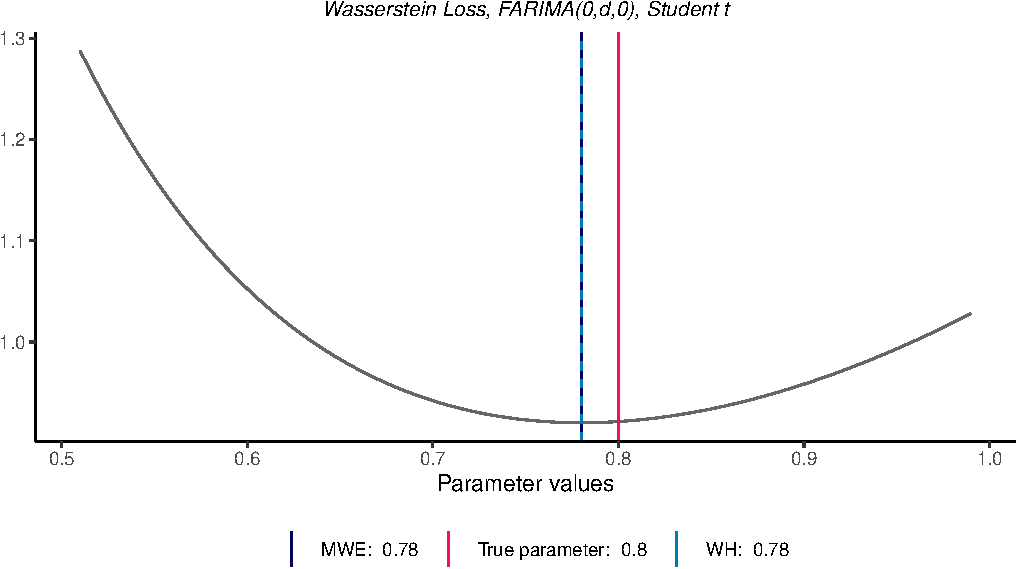
\includegraphics[width=0.5\linewidth]{Master_thesis_V4_files/figure-latex/Student_t-1} 

}

\caption{Wasserstein loss function of a FARIMA(0,d,0) process distributed according to a Student t distribution with degree of freedom equal to 4. The sample size is equal to 3001.}\label{fig:Student_t}
\end{figure}

In addition to modifying the excess of kurtosis of a distribution and
thus increasing the probability of observing extreme values, we are also
interested in observing how our estimators behave when the error
distribution is asymmetric. Therefore, we use the skew normal
distribution \(SN(\alpha)\) to allow for non-zero skewness by varying
the symmetry parameter \(\alpha\) of the distribution. Then, we combine
these two descriptive statistics of the errors distribution through the
skew t distribution recently developed by
\protect\hyperlink{ref-azzalini2003distributions}{Azzalini and
Capitanio} (\protect\hyperlink{ref-azzalini2003distributions}{2003}).
Consequently, the distribution of the innovation terms becomes heavy
tailed but on top of that skewed.

The skew t distribution is related to a standard skew normal random
variable \(T\) and a random variable \(M\) following a chi-squared
distribution with \(\mathrm{v}\) degree of freedom by the equation:

\[R=\frac{T}{\sqrt{\frac{M}{\mathrm{v}}}}.\]

Then the linear transformation \(X=\mu+\sigma R\) has a skew t
distribution with parameters \(\mu, \sigma, \alpha\), and \(\mathrm{v}\)
and the corresponding notation
\(S T(\mu = 0, \sigma = 1, \alpha, \mathrm{v})\) to denote the skew t
random variable \(X\).

For illustration, we plot on Figure \ref{fig:skewt_density} densities of
skew normal and skew t distribution for some selected values of
\(\alpha\) and \(\mathrm{v}\).

\begin{figure}

{\centering 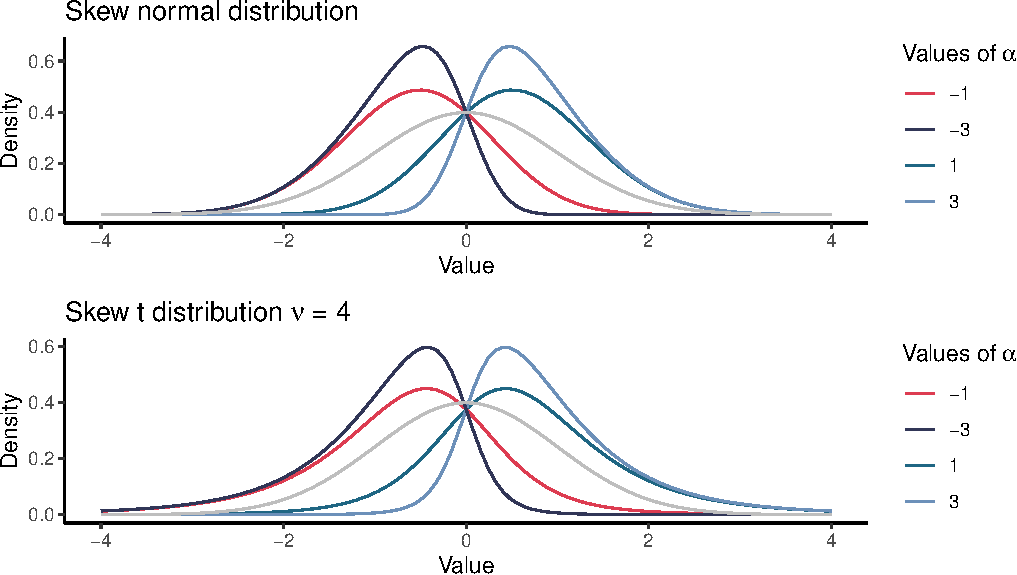
\includegraphics[width=0.65\linewidth]{Master_thesis_V4_files/figure-latex/skewt_density-1} 

}

\caption{Density plot of skew normal and skew t distribution for some selected values of the skewness parameter and the degree of freedom.}\label{fig:skewt_density}
\end{figure}

In order to compare our estimators fairly in our Monte Carlo
simulations, we keep the parameters of these three distributions
constant. Therefore, we consider a Student t distribution with a degree
of freedom equal to 4, i.e \(\epsilon_t \sim t_{\mathrm{v} =4}\), a skew
normal distribution with shape parameter equal to 1,
i.e.~\(\epsilon_t \sim SN(\alpha = 1)\) and a skew t distribution
combining both of them,
i.e.~\(\epsilon_t \sim S T(\mu = 0, \sigma = 1, \alpha = 1, \mathrm{v} = 4)\).

We simulate \(B = 400\) FARIMA(0,d,0) processes for each of these three
distributions and plot the result on Figure \ref{fig:box_farima_full}.

Let us begin by analyzing what occurs when the distribution is a Student
t (top plot of Figure \ref{fig:box_farima_full}). We note that all
estimators (apart from those based on the Sinkhorn distance) have a
considerably smaller variance than when the process is Gaussian and,
consequently, a smaller MSE (see Table \ref{tab:mse_farima}). For
example, the first and third quartile of the minimum semidiscrete
Wasserstein estimator are respectively \(0.758\) and \(0.832\) in the
case of Gaussian processes and becomes \(0.788\) and \(0.8089\) when the
distribution has heavier tails. The Whittle's estimator remains the
leader in terms of MSE.

Then, when the distribution is set to be a skew normal one, we can
notice that a bias arises for each estimators (see middle plot of Figure
\ref{fig:box_farima_full}). Indeed, all estimators are biased in the
sense they overestimate the value of the parameter. The Whittle's
estimator is the second estimator that suffers most from this bias. Our
new estimators are more robust and subsequently experience a smaller MSE
(see Table \ref{tab:mse_farima}).

Regarding the impact of the skew t distribution, all the MSE are better
than when the distribution is simply asymmetric due to the fact that
having heavier tails seems to make the estimators converge faster.

To sum up, the estimators based on the Wasserstein distance (expect for
the minimum weighted Wasserstein estimator) overperform the Whittle's
estimator when the underlying distribution of the innovation terms is
skewed.

\begin{figure}

{\centering \includegraphics[width=0.75\linewidth]{/Users/manonfelix/OneDrive/Master thesis/Redaction/images/FARIMA_full} 

}

\caption{Boxplots of all the estimators presented during this thesis. The sample size of the 200 simulated FARIMA(0,d,0) is 3201. From top to bottom the underlying distrubtions are Student t, skew normal and skew t.}\label{fig:box_farima_full}
\end{figure}

\begin{table}[]
\centering
\begin{tabular}{|l|c|c|c|}
\hline
\multicolumn{1}{|c|}{\textbf{FARIMA($0,d = 0.3,0$)}}          & $\widehat{MSE}( \hat \theta^*)$ & $\widehat{Bias}( \hat \theta^*)$ & $\widehat{Var}( \hat \theta^*)$ \\ \hline
\multicolumn{1}{|c|}{\textbf{Distribution}}                   & \multicolumn{3}{c|}{\textbf{Student t}}                             \\ \hline
$\hat \theta^*_{Whittle}$                                     & 0.000211             & -0.001675             & 0.000210             \\ \hline
$\hat \theta^*_{MWE}$                                         & 0.002846             & 0.012169              & 0.002712             \\ \hline
$\hat \theta^*_{MMWE, \ k = 50}$                              & 0.000314             & 0.003980              & 0.000300             \\ \hline
$\hat \theta^*_{MSWE}$                                        & 0.000214             & -0.001689             & 0.000212             \\ \hline
$\hat \theta^*_{MWWE}$                                        & 0.000295             & -0.002362             & 0.000290             \\ \hline
$\hat \theta^*_{MSKE, \ \lambda = 0.1}$                       & 0.000570             & -0.000891             & 0.000572             \\ \hline
$\hat \theta^*_{MSKE, \ \lambda = 0.3}$                       & 0.001287             & 0.024379              & 0.000696             \\ \hline
\multicolumn{1}{|c|}{\textbf{Distribution}}                   & \multicolumn{3}{c|}{\textbf{Skew normal}}                           \\ \hline
$\hat \theta^*_{Whittle}$                                     & 0.020847             & 0.143981              & 0.000117             \\ \hline
$\hat \theta^*_{MWE}$                                         & 0.006300             & 0.069800              & 0.001435             \\ \hline
$\hat \theta^*_{MMWE, \ k = 50}$                              & 0.009379             & 0.091769              & 0.000963             \\ \hline
$\hat \theta^*_{MSWE}$                                        & 0.008979             & 0.085507              & 0.001676             \\ \hline
$\hat \theta^*_{MWWE}$                                        & 0.025578             & 0.159484              & 0.000144             \\ \hline
$\hat \theta^*_{MSKE, \ \lambda = 0.1}$                      & 0.011437             & 0.105650              & 0.000277             \\ \hline
$\hat \theta^*_{MSKE, \ \lambda = 0.3}$                       & 0.018244             & 0.133753              & 0.000356             \\ \hline
\multicolumn{1}{|c|}{\textbf{Distribution}}                   & \multicolumn{3}{c|}{\textbf{Skew t}}                                \\ \hline
$\hat \theta^*_{Whittle}$                                     & 0.014959             & 0.121619              & 0.000169             \\ \hline
$\hat \theta^*_{MWE}$                                         & 0.008616             & 0.087040              & 0.001045             \\ \hline
$\hat \theta^*_{MMWE, \ k = 50}$                              & 0.009343             & 0.093530              & 0.000598             \\ \hline
$\hat \theta^*_{MSWE}$                                        & 0.013206             & 0.114045              & 0.000201             \\ \hline
$\hat \theta^*_{MWWE}$                                        & 0.020252             & 0.141760              & 0.000157             \\ \hline
$\hat \theta^*_{MSKE, \ \lambda = 0.1}$                        & 0.008096             & 0.088171              & 0.000324             \\ \hline
$\hat \theta^*_{MSKE, \ \lambda = 0.3}$                       & 0.014119             & 0.117058              & 0.000418             \\ \hline
\end{tabular}
\caption{MSE, bias and variance computed with 200 simulated FARIMA(0,d,0) processes with three different underlying distributions.}
\label{tab:mse_farima}
\end{table}

\pagebreak

\hypertarget{additive-outliers-long-memory}{%
\subsubsection{Additive Outliers :
Long-Memory}\label{additive-outliers-long-memory}}

In the presence of contamination in the time series (e.g.~additive
outliers). For example, in the case of Gaussian FARIMA(0, d, 0) some of
our estimators (in particular, the one based on weighted Wasserstein
distance) seem to overperform Whittle's estimator in terms of MSE. To
demonstrate this propriety we simulate \(mt = 200\) FARIMA(\(0,d,0\))
contaminated by occasional isolated outliers. The gaussian processes
\(\{Y_t\}\) are distributed according to

\[Y_{t}=\left(1-W_{t}\right) X_{t}+W_{t}\left(c \cdot V_{t}\right)\]
where \(W_t \sim Bern(p)\), \(V_t \sim t_2\) and c = 10. In Table
\ref{tab:outliers}, we report the ratio between the MSE / bias /
variance of the Whittle's estimator and the minimum weighted Wasserstein
estimator for different values of \(p = 0, 0.001, 0.01, 0.05\) (when
\(p = 0\) the process is not contaminated by outliers). The results
suggest that when the time series is contaminated, the minimum weighted
Wasserstein estimator overperform the Whittle's estimator in terms of
MSE. Indeed, as soon as we introduce noise the ratio becomes greater
than \(1\). For a \(p < 0.01\), we improve the bias and the variance
thanks to the weights and when \(p \geq 0.01\) our gain exclusively
comes from the bias.

\begin{table}[h]
\centering
\begin{tabular}{|c|c|c|c|c|}
\hline
p  &  0  & 0.001   & 0.01    & 0.05 \\
\hline
MSE ratio  & 0.682 & 1.208 & 1.105 & 1.012 \\
\hline
Bias ratio & 0.104 & 1.000 & 1.054 & 1.010\\
\hline 
Variance ratio & 0.686 & 1.206 & 0.991 & 0.8128 \\ 
\hline
\end{tabular}
\caption{MSE / Bias / Variance of the Whittle's estimator divided by the MSE / bias / varaince of the MWWE. The number of simulated time series is equal to 200 with sample size equal to 3001. The innovation terms are distributed according to a standard normal distribution.}
\label{tab:outliers}
\end{table}

\hypertarget{short-memory-process}{%
\subsubsection{Short-memory Process}\label{short-memory-process}}

We also aim to demonstrate the performance of our estimators for
short-memory processes. To do this, we simulate \(B = 200\)
auto-regressive processes of order 2 according to:

\[Y_t = 0.75 Y_{t-1} - 0.25Y_{t-2} + \epsilon_t.\]

The processes are stationary since the three stationary conditions are
met:

\begin{enumerate}
\def\labelenumi{\arabic{enumi}.}
\tightlist
\item
  \(\phi_{2}<1+\phi_{1}\)
\item
  \(\phi_{2}<1-\phi_{1}\)
\item
  \(\phi_{2}>-1\)
\end{enumerate}

where \(\phi_1 = 0.75\) and \(\phi_2 = -0.25\).

We cannot include the Sinkhorn divergence in our comparison because the
function used on R requires too much time to calculate this divergence
and fails to converge. The results when
\(\theta^* \subset \mathbb{R}^2\) are on Figure \ref{fig:ar2_full} with
corresponding MSE, bias and variance for each estimator in Table
\ref{tab:AR2_gaussian_table}, \ref{tab:AR2_Student_table},
\ref{tab:AR2_skew_normal_table} and \ref{tab:AR2_skew_t_table}. Again,
we consider several distributions for \(\epsilon_t\):
\(\epsilon_t \sim N(0,1), \epsilon_t \sim t_4\),
\(\epsilon_t \sim SN(\alpha = 1)\) and
\(\epsilon_t \sim S T(\mu = 0, \sigma = 1, \alpha = 1, \mathrm{v} = 4)\).
The corresponding boxplots of all the simulations are presented on
Figure \ref{fig:ar2_full}.

\begin{figure}

{\centering \includegraphics[width=1\linewidth]{/Users/manonfelix/OneDrive/Master thesis/Redaction/images/AR2_full} 

}

\caption{Boxplots of the Whittle's estimator, MWE, MSWE, MMWE, MWWE for 200 AR(2) processes. The left column is the first parameter (0.75) of the process, the right one is for the second parameter (-0.25).}\label{fig:ar2_full}
\end{figure}

First, we consider Gaussian AR(\(2\)) processes,
i.e.~\(\epsilon_t \sim N(0,1)\). The Whittle's estimator always scores
better in terms of MSE, bias and variance for both parameters (see Table
\ref{tab:AR2_gaussian_table}). The estimator with results roughly
similar to the state-of-the art estimator is the minimum weighted
Wasserstein estimator. Unlike the others which have a high variance and,
consequently, a high MSE.

\begin{table}[h]
\centering
\begin{tabular}{|l|c|c|c|c|c|c|}
\hline
\multicolumn{1}{|c|}{\textbf{Distribution}} & \multicolumn{6}{c|}{\textbf{Gaussian}}                                                                                                                           \\ \hline
\textbf{}                                   & \multicolumn{2}{c|}{$\widehat{MSE}( \hat \theta^*)$} & \multicolumn{2}{c|}{$\widehat{Bias}( \hat \theta^*)$} & \multicolumn{2}{c|}{$\widehat{Var}( \hat \theta^*)$} \\ \hline
                                            & $\phi_1$                 & $\phi_2$                 & $\phi_1$                  & $\phi_2$                 & $\phi_1$                 & $\phi_2$                 \\ \hline
$\hat \theta^*_{Whittle}$                   & 0.000279                  & 0.000308                  & -0.001944                  & 0.000154                  & 0.000276                  & 0.000309                  \\ \hline
$\hat \theta^*_{MWE}$                       & 0.005119                  & 0.007030                  & -0.012938                  & 0.030338                  & 0.004964                  & 0.006125                  \\ \hline
$\hat \theta^*_{MMWE, \ k = 50}$            & 0.003132                  & 0.003166                  & -0.007961                  & 0.011897                  & 0.003077                  & 0.003032                  \\ \hline
$\hat \theta^*_{MSWE}$                      & 0.003974                  & 0.004072                  & -0.010912                  & 0.013176                  & 0.003864                  & 0.003909                  \\ \hline
$\hat \theta^*_{MWWE}$                      & 0.000383                  & 0.000449                  & -0.002598                  & 0.000442                  & 0.000377                  & 0.000450                  \\ \hline
\end{tabular}
\caption{Mean Squared Error / Bias / Variance of Figure 16 top plots.}
\label{tab:AR2_gaussian_table}
\end{table}

In the scenario where the process distribution is heavy tailed, here
Student t distribution, all MSE values of our new estimators decrease
(see Table \ref{tab:AR2_Student_table}). As we can see on Figure
\ref{fig:ar2_full}, the boxplots cluster much more around the true
value. As before, estimators converge faster to the true value of the
parameter when the probability of getting very large values is higher
than the standard normal distribution. The Whittle's estimator continues
to achieve the best performance in terms of MSE.

\begin{table}[h]
\centering
\begin{tabular}{|l|c|c|c|c|c|c|}
\hline
\multicolumn{1}{|c|}{\textbf{Distribution}} & \multicolumn{6}{c|}{\textbf{Student t}}                                                                                                                          \\ \hline
\textbf{}                                   & \multicolumn{2}{c|}{$\widehat{MSE}( \hat \theta^*)$} & \multicolumn{2}{c|}{$\widehat{Bias}( \hat \theta^*)$} & \multicolumn{2}{c|}{$\widehat{Var}( \hat \theta^*)$} \\ \hline
                                            & $\phi_1$                 & $\phi_2$                 & $\phi_1$                  & $\phi_2$                 & $\phi_1$                 & $\phi_2$                 \\ \hline
$\hat \theta^*_{Whittle}$                   & 0.000321                  & 0.000281                  & -0.00117                  & -0.001100                  & 0.000321                  & 0.000281                  \\ \hline
$\hat \theta^*_{MWE}$                       & 0.002953                  & 0.003386                  & -0.005827                   & 0.014389                 & 0.002934                  & 0.003195                  \\ \hline
$\hat \theta^*_{MMWE, \ k = 50}$            & 0.000612                  & 0.000586                  & -0.000508                  & -0.001591                  & 0.000615                  & 0.000586                  \\ \hline
$\hat \theta^*_{MSWE}$                      & 0.000324                  & 0.000281                  & -0.001093                  & -0.001109                  & 0.000325                  & 0.000281                  \\ \hline
$\hat \theta^*_{MWWE}$                      & 0.000438                  & 0.000400                  & -0.001415                  & -0.000151                  & 0.000438                  & 0.000402                  \\ \hline
\end{tabular}
\caption{Mean Squared Error / Bias / Variance of Figure 16 second plot from the top.}
\label{tab:AR2_Student_table}
\end{table}

On the other hand, contrary to long-memory processes, we observe that
the fact that the underlying distribution are skewed or not is not
relevant during the estimation procedure of the Whittle's estimator.
Indeed, we do not perceive any bias in the Whittle's estimator in Figure
\ref{fig:ar2_full} (third plot from the top) which is confirmed in Table
\ref{tab:AR2_skew_normal_table}. Regarding the estimators based on the
Wasserstein distance we can observe a bias when the underlying
distribution is a skew normal one. As soon as we raise the kurtosis of
the distribution by means of the skew t distribution this bias
disappears (see the bottom plot of Figure \ref{fig:ar2_full} and Table
\ref{tab:AR2_skew_t_table}). As for the minimum weighted Wasserstein
estimator, it remains consistent with the Whittle's estimator and is
always very similar to it.

\begin{table}[h]
\centering
\begin{tabular}{|l|c|c|c|c|c|c|}
\hline
\multicolumn{1}{|c|}{\textbf{Distribution}} & \multicolumn{6}{c|}{\textbf{Skew normal}}                                                                                                                          \\ \hline
\textbf{}                                   & \multicolumn{2}{c|}{$\widehat{MSE}( \hat \theta^*)$} & \multicolumn{2}{c|}{$\widehat{Bias}( \hat \theta^*)$} & \multicolumn{2}{c|}{$\widehat{Var}( \hat \theta^*)$} \\ \hline
                                            & $\phi_1$                 & $\phi_2$                 & $\phi_1$                  & $\phi_2$                 & $\phi_1$                 & $\phi_2$                 \\ \hline
$\hat \theta^*_{Whittle}$                   & 0.000269                  & 0.000258                  & -0.001515                  & 0.000316                  & 0.000268                  & 0.000257                  \\ \hline
$\hat \theta^*_{MWE}$                       & 0.214071                  & 0.131399                  & -0.452852                   & 0.355448                 & 0.009041                  & 0.000554                  \\ \hline
$\hat \theta^*_{MMWE, \ k = 50}$            & 0.218021                  & 0.141375                  & -0.454870                  & 0.371929                  & 0.011169                  & 0.003059                  \\ \hline
$\hat \theta^*_{MSWE}$                      & 0.220240                  & 0.136362                  & -0.446864                  & 0.363478                  & 0.020656                  & 0.004267                  \\ \hline
$\hat \theta^*_{MWWE}$                      & 0.000548                  & 0.000554                  & -0.000497                  & -0.000933                  & 0.000546                  & 0.0.000552                  \\ \hline
\end{tabular}
\caption{Mean Squared Error / Bias / Variance of Figure 16 third plot from the top.}
\label{tab:AR2_skew_normal_table}
\end{table}

\begin{table}[h]
\centering
\begin{tabular}{|l|c|c|c|c|c|c|}
\hline
\multicolumn{1}{|c|}{\textbf{Distribution}} & \multicolumn{6}{c|}{\textbf{Skew t}}                                                                                                                          \\ \hline
\textbf{}                                   & \multicolumn{2}{c|}{$\widehat{MSE}( \hat \theta^*)$} & \multicolumn{2}{c|}{$\widehat{Bias}( \hat \theta^*)$} & \multicolumn{2}{c|}{$\widehat{Var}( \hat \theta^*)$} \\ \hline
                                            & $\phi_1$                 & $\phi_2$                 & $\phi_1$                  & $\phi_2$                 & $\phi_1$                 & $\phi_2$                 \\ \hline
$\hat \theta^*_{Whittle}$                   & 0.000321                  & 0.000306                  & -0.001068                  & -0.000779                  & 0.000321                  & 0.000307                  \\ \hline
$\hat \theta^*_{MWE}$                       & 0.003282                  & 0.005058                  & -0.009552                   & 0.021269                 & 0.003206                  & 0.004629                  \\ \hline
$\hat \theta^*_{MMWE, \ k = 50}$            & 0.000705                  & 0.000634                  & -0.000656                  & -0.000937                  & 0.000708                  & 0.000634                  \\ \hline
$\hat \theta^*_{MSWE}$                      & 0.000319                  & 0.000303                  & -0.001133                  & -0.000854                  & 0.000319                  & 0.000304                  \\ \hline
$\hat \theta^*_{MWWE}$                      & 0.000373                  & 0.000397                  & -0.000370                  & -0.001441                  & 0.000375                  & 0.000398                  \\ \hline
\end{tabular}
\caption{Mean Squared Error / Bias / Variance of Figure 16 bottom plot.}
\label{tab:AR2_skew_t_table}
\end{table}

In order to explain why a bias appears when
\(\epsilon_t \sim SN(\alpha)\) and does not appear when we consider
\(\epsilon_t \sim ST(\alpha, \mathrm{v})\), we compute the Wasserstein
loss of an AR(1) process \(Y_t = \phi_1 Y_{t-1} + \epsilon_t\) where
\(\phi_1 = 0.6\) and \(\epsilon_t \sim SN(\alpha = 0.1)\) in the left
plot of Figure \ref{fig:AR1_loss} and
\(\epsilon_t \sim ST(\alpha = 0.1, \mathrm{v} = 4)\) in the right plot.
By introducing an excess of kurtosis, thanks to the skew t distribution,
we are facing a smooth Wasserstein loss. The convexe shape of the
Wasserstein loss around the minimum value (see Figure \ref{fig:AR1_loss}
left plot) in the case of a skew normal distribution induces a bias in
the parameter estimation.

\begin{figure}

{\centering 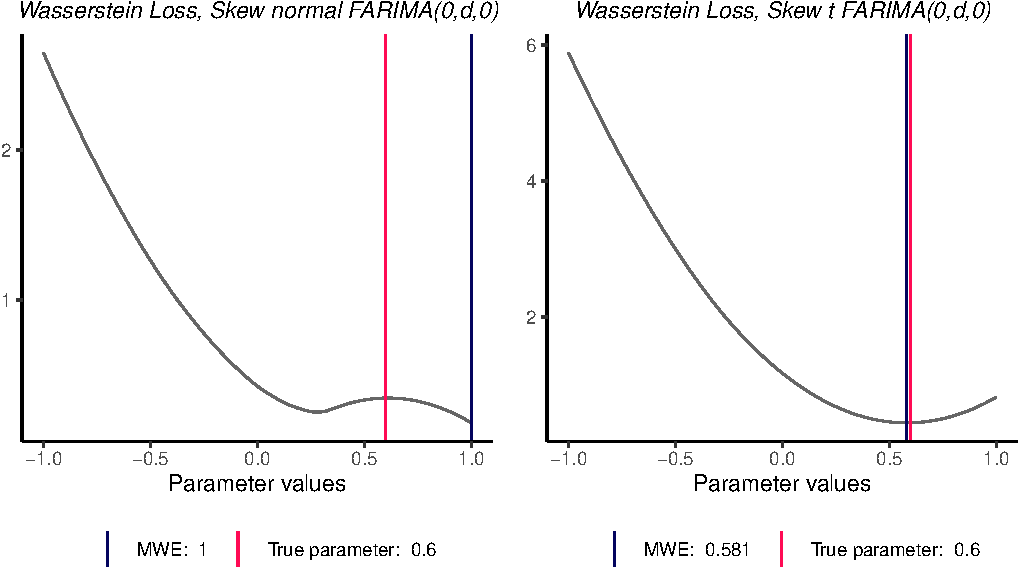
\includegraphics[width=0.75\linewidth]{Master_thesis_V4_files/figure-latex/AR1_loss-1} 

}

\caption{Wasserstein loss function of two AR(1) process with underlying distribution being a skew normal distribution and a skew t distribution. The sample size is equal to 3001}\label{fig:AR1_loss}
\end{figure}

\hypertarget{additive-outliers-short-memory}{%
\subsubsection{Additive Outliers :
Short-Memory}\label{additive-outliers-short-memory}}

We also replicate our experiment presented above by introducing some
occasional outliers in a Gaussian AR(1) process

\[Y_t = 0.6Y_{t-1} + \epsilon_t\]

As a reminder, we contaminate the \(200\) simulated processes by means
of the following equation:

\[Y_{t}=\left(1-W_{t}\right) X_{t}+W_{t}\left(c \cdot V_{t}\right)\]

where \(W_t \sim Bern(p)\), \(V_t \sim t_2\) and \(c = 10\). We let the
value of \(p\) vary and evaluate the performance with three different
ratios between the Whittle's estimator and the minimum weighted
Wasserstein estimator: MSE ratio, bias ratio and variance ratio. The
results are listed in Table \ref{tab:outliers_AR1}. We observe the same
kind of effect as for the long-memory process. Indeed, our minimum
weighted Wasserstein estimator outperforms the Whittle's estimator when
the process is contaminated. This improvement is due to the bias and
variance both being smaller for the minimum weighted Wasserstein
estimator for \(p <0.05\). Then, when \(p \geq 0.05\), the minimum
weighted Wasserstein estimator has a larger variance than the Whittle's.

\begin{table}[h]
\centering
\begin{tabular}{|c|c|c|c|c|}
\hline
p  &  0  & 0.001   & 0.01    & 0.05 \\
\hline
MSE ratio  & 0.753 & 1.282 & 1.089 & 1.010 \\
\hline
Bias ratio & 0.905 & 1.107 & 1.044 & 1.005\\
\hline 
Variance ratio & 0.749 & 1.327 & 1.0589 & 0.813 \\ 
\hline
\end{tabular}
\caption{MSE / Bias / Variance of the Whittle's estimator divided by the MSE / bias / variance of the MWWE. The number of simulated AR(1) processes is equal to 200 with sample size equal to 3001. The innovation terms are distributed according to a standard normal distribution.}
\label{tab:outliers_AR1}
\end{table}

\hypertarget{conclusion}{%
\section{Conclusion}\label{conclusion}}

In this thesis, we introduce five new estimators that are based on
minimum distance/divergence estimation. Our results suggest that we can
outperform the state-of-the art estimation procedure when we are dealing
with long-memory processes that have skewed underlying distributions.
Moreover, it seems that our minimum weighted Wasserstein estimator can
also be more efficient when short- and long-memory processes are
contaminated by occasional outliers. In the case of short memory
processes, we have similar results to Whittle's estimator in terms of
MSE. Through this thesis, we open the possibility for further research
directions. An important step is to provide the theoretical
understanding of our novel estimators, studying e.g., consistency,
asymptotic normality and robustness.

\newpage

\hypertarget{references}{%
\section*{References}\label{references}}
\addcontentsline{toc}{section}{References}

\hypertarget{refs}{}
\begin{CSLReferences}{1}{0}
\leavevmode\hypertarget{ref-ambrosio2013user}{}%
Ambrosio, Luigi, and Nicola Gigli. 2013. {``A User's Guide to Optimal
Transport.''} In \emph{Modelling and Optimisation of Flows on Networks},
1--155. Springer.

\leavevmode\hypertarget{ref-arjovsky2017wasserstein}{}%
Arjovsky, Martin, Soumith Chintala, and Léon Bottou. 2017.
{``Wasserstein Generative Adversarial Networks.''} In
\emph{International Conference on Machine Learning}, 214--23. PMLR.

\leavevmode\hypertarget{ref-azzalini2003distributions}{}%
Azzalini, Adelchi, and Antonella Capitanio. 2003. {``Distributions
Generated by Perturbation of Symmetry with Emphasis on a Multivariate
Skew t-Distribution.''} \emph{Journal of the Royal Statistical Society:
Series B (Statistical Methodology)} 65 (2): 367--89.

\leavevmode\hypertarget{ref-bassetti2006minimum}{}%
Bassetti, Federico, Antonella Bodini, and Eugenio Regazzini. 2006. {``On
Minimum Kantorovich Distance Estimators.''} \emph{Statistics \&
Probability Letters} 76 (12): 1298--1302.

\leavevmode\hypertarget{ref-basu2019statistical}{}%
Basu, Ayanendranath, Hiroyuki Shioya, and Chanseok Park. 2019.
\emph{Statistical Inference: The Minimum Distance Approach}. Chapman;
Hall/CRC.

\leavevmode\hypertarget{ref-beran1994statistics}{}%
Beran, Jan. 1994. \emph{Statistics for Long-Memory Processes}. Vol. 61.
CRC press.

\leavevmode\hypertarget{ref-bernton2019parameter}{}%
Bernton, Espen, Pierre E Jacob, Mathieu Gerber, and Christian P Robert.
2019. {``On Parameter Estimation with the Wasserstein Distance.''}
\emph{Information and Inference: A Journal of the IMA} 8 (4): 657--76.

\leavevmode\hypertarget{ref-brillinger2001time}{}%
Brillinger, David R. 2001. \emph{Time Series: Data Analysis and Theory}.
SIAM.

\leavevmode\hypertarget{ref-cuturi2013sinkhorn}{}%
Cuturi, Marco. 2013. {``Sinkhorn Distances: Lightspeed Computation of
Optimal Transport.''} \emph{Advances in Neural Information Processing
Systems} 26: 2292--2300.

\leavevmode\hypertarget{ref-friedman2001elements}{}%
Friedman, Jerome, Trevor Hastie, Robert Tibshirani, and others. 2001.
\emph{The Elements of Statistical Learning}. Vol. 1. 10. Springer series
in statistics New York.

\leavevmode\hypertarget{ref-gourieroux1995statistics}{}%
Gourieroux, Christian, and Alain Monfort. 1995. \emph{Statistics and
Econometric Models}. Vol. 1. Cambridge University Press.

\leavevmode\hypertarget{ref-kantorovich1942translocation}{}%
Kantorovich, Leonid V. 1942. {``On the Translocation of Masses.''} In
\emph{Dokl. Akad. Nauk. USSR (NS)}, 37:199--201.

\leavevmode\hypertarget{ref-kolouri2017optimal}{}%
Kolouri, Soheil, Se Rim Park, Matthew Thorpe, Dejan Slepcev, and Gustavo
K Rohde. 2017. {``Optimal Mass Transport: Signal Processing and
Machine-Learning Applications.''} \emph{IEEE Signal Processing Magazine}
34 (4): 43--59.

\leavevmode\hypertarget{ref-mikosch1995parameter}{}%
Mikosch, Thomas, Tamar Gadrich, Claudia Kluppelberg, and Robert J Adler.
1995. {``Parameter Estimation for ARMA Models with Infinite Variance
Innovations.''} \emph{The Annals of Statistics}, 305--26.

\leavevmode\hypertarget{ref-monge1781memoire}{}%
Monge, Gaspard. 1781. {``M{é}moire Sur La Th{é}orie Des d{é}blais Et Des
Remblais.''} \emph{Histoire de l'Acad{é}mie Royale Des Sciences de
Paris}.

\leavevmode\hypertarget{ref-ni2020conditional}{}%
Ni, Hao, Lukasz Szpruch, Magnus Wiese, Shujian Liao, and Baoren Xiao.
2020. {``Conditional Sig-Wasserstein GANs for Time Series Generation.''}
\emph{arXiv Preprint arXiv:2006.05421}.

\leavevmode\hypertarget{ref-panaretos2020invitation}{}%
Panaretos, Victor M, and Yoav Zemel. 2020. \emph{An Invitation to
Statistics in Wasserstein Space}. Springer Nature.

\leavevmode\hypertarget{ref-peyre2019computational}{}%
Peyré, Gabriel, Marco Cuturi, and others. 2019. {``Computational Optimal
Transport: With Applications to Data Science.''} \emph{Foundations and
Trends in Machine Learning} 11 (5-6): 355--607.

\leavevmode\hypertarget{ref-priestley1981spectral}{}%
Priestley, Maurice Bertram. 1981. \emph{Spectral Analysis and Time
Series: Probability and Mathematical Statistics}. 04; QA280, P7.

\leavevmode\hypertarget{ref-santambrogio2015optimal}{}%
Santambrogio, Filippo. 2015. {``Optimal Transport for Applied
Mathematicians.''} \emph{Birk{ä}user, NY} 55 (58-63): 94.

\leavevmode\hypertarget{ref-tsay2005analysis}{}%
Tsay, Ruey S. 2005. \emph{Analysis of Financial Time Series}. Vol. 543.
John wiley \& sons.

\leavevmode\hypertarget{ref-villani2009optimal}{}%
Villani, Cédric. 2009. \emph{Optimal Transport: Old and New}. Vol. 338.
Springer.

\leavevmode\hypertarget{ref-whittle1953estimation}{}%
Whittle, Peter. 1953. {``Estimation and Information in Stationary Time
Series.''} \emph{Arkiv f{ö}r Matematik} 2 (5): 423--34.

\end{CSLReferences}

\end{document}
